\section{Outline}\label{outline}

\begin{enumerate}
\def\labelenumi{\arabic{enumi}.}
\setcounter{enumi}{-1}
\tightlist
\item
  Abstract
\item
  Introduction
\item
  Model

  \begin{itemize}
  \tightlist
  \item
    2.1 agent based model, introduced textually
  \item
    2.2 branching process
  \item
    2.3 integro differential
  \item
    2.4 difference
  \end{itemize}
\item
  Results

  \begin{itemize}
  \tightlist
  \item
    3.1 Extinction Probability
  \item
    3.2 Max I, Total R
  \item
    3.3 Disease Evolution
  \end{itemize}
\item
  Discussion
\item
  Appendix

  \begin{itemize}
  \tightlist
  \item
    A.1 branching process derivations
  \item
    A.2 differential equations - moments
  \item
    A.3 basic reproduction number
  \item
    A.4 differential equations - mean riskyness results
  \item
    A.5 choice of \(\gamma\) and \(N\)
  \item
    A.6 model comparisons
  \end{itemize}
\end{enumerate}

\section{0. Abstract}\label{abstract}

Disease transmission is often not homogeneous: a small number of
infected individuals are responsible for a disproportionately large
number of subsequent infections.

This is certainly the case in COVID-19, in which 20\% of infections may
cause as many as 80\% of secondary infections{[}citation?{]}. However,
our mechanistic understanding of this phenomenon -- ``super-spreading''
-- is limited{[}citations?{]}.

Here we introduce and analyze a model of an outbreak with
super-spreading via ``problem-place'' locations: disease spreads
homogeneously throughout the population at a low rate, but spreads
rampantly at certain locations (bars, restaurants, churches, etc.) that
individuals visit daily with their own fixed probabilities.

Compared to homogeneous dynamics, outbreaks are less likely to happen
but are accelerated when they do occur; causing larger outbreaks in some
cases, but paradoxically smaller and less severe outbreaks in moderately
to highly infectious diseases.

\section{1. Introduction}\label{introduction}

After the SARS pandemic in 2005, researchers noted that disease
transmission was not homogeneous: some small number of infected
individuals -- ``super spreaders'' -- were responsible for a
disproportionately large number of total infections.{[}2005 nature
citation{]} Subsequent research noted a similar pattern in other
diseases: between 15\% to 20\% of infected individuals caused 75\% to
85\% of infections in diseases as diverse as (\emph{add examples from
2006 paper}). {[}2006 super spreading{]}. The COVID-19 pandemic follows
a similar pattern: 15\% of super-spreading- infected individuals cause
80\% of later infections.

However, research into the dynamics of disease outbreaks with
superspreading has been mostly limited to models in which some
individuals are simply more infectious -- either because of greater
biological infectiousness (higher viral load, larger lung capacity,
etc.) or greater network connectivity. But this doesn't match what we
understand about the COVID-19 pandemic. Firstly, individual
infectiousness doesn't vary all that much {[}citation of this{]}. And
while much can be learned from a model that simply assumes some
individuals have many more social connections than others, this misses
the crucial and salient fact that COVID transmission is centered around
certain ``hot spots'' (bars, restaurants, churches, etc) {[}problem
place paper{]}. We'd like to understand how the picture changes when
disease spreads largely (or even primarily) through certain ``hot
spots'' and the most important predictive variable of an individual's
superspreading capability is their likeilihood to visit such a hot spot
over any given time interval.

To address this missing piece, we introduce the ``hot-spot'' SIR model.
This model is risk-structured: each individual has a fixed probability
(riskyness) of visiting a ``hot spot'' per unit time, where disease
spreads with very high transmission rate between all present
individuals, and simultaneously is subject to ``community spread'' which
acts homogeneously between all individuals with much low transmission
rate. We find that with these dynamics, initial outbreaks in a fixed
population where one individual becomes infected happen much less
readily (for comparable overall transmission rates). Similar to previous
work, {[}heterogeneous spread citation, SSE papers{]} we find that when
there is an outbreak it occurs much faster or ``explosively''. However,
we also see the outbreak die out much more rapidly -- due to the average
riskiness in the infected and susceptible populations both declining
after a point. Surprisingly, this leads to explosive outbreaks that
nevertheless infect fewer people both overall and at their peak over a
fairly wide range of average disease infectiousness (defined below).

\section{2. Methods}\label{methods}

We first consider an agent-based model.

\subsection{2.1 Agent-based (simulation)
model}\label{agent-based-simulation-model}

\subsubsection{Setup}\label{setup}

We initialize a fixed-size population of \(N\) agents. Each agent \(i\)
(\(i \in [0, N)\)) is characterized by a fixed ``riskyness'' parameter
\(\rho_i \in [0, 1]\) that never changes, and a disease state of
Susceptible (S), Infected (I) or Recovered (R). We set the following
parameters:

\begin{itemize}
\tightlist
\item
  \(\beta_c \in [0, 1], << 1\) community spread rate -- the probability
  of disease spreading from an I to an S individual through a single
  community contact,
\item
  \(\beta_p \in [0, 1], << 1\) hot-spot spread rate - the probability of
  disease spreading from an I to an S individual through contact in the
  problem-place; this is typically larger than \(\beta_c\).
\item
  \(\gamma \in (0, 1]\) the recovery rate - the rate at which I
  individuals move to R (the disease lasts on average \(1/\gamma\) time
  units).
\end{itemize}

All agents \(i\) are initially S, and each's \(\rho_i\) is drawn iid.
from a specific fixed distribution \(\mathrm{P}\) over \([0, 1]\). One
agent is chosen at random and set to I to start the simulation.

\subsubsection{Dynamics}\label{dynamics}

\paragraph{Risk Taking}\label{risk-taking}

Every timestep, each agent \(i\) visits the problem place with
probability \(\rho_i\).

\paragraph{Disease Spread}\label{disease-spread}

All agents in the problem place make a contact with all other agents in
the problem place; I individuals in this subset spread the disease to S
individuals with probability \(\beta_p\) (problem place spread).
Simultaneously, all agents (in and out of the problem place) make
contact with all other agents and (I) individuals spread to (S)
individuals with probability \(\beta_c\) (homogeneous community spread).

\paragraph{Recovery}\label{recovery}

\begin{enumerate}
\def\labelenumi{(\Roman{enumi})}
\tightlist
\item
  agents recover with probability \(\gamma\). If there are no (I)
  agents, the simulation ends.
\end{enumerate}

\subsection{2.2 Investigation Procedure}\label{investigation-procedure}

To investigate how disease dynamics and outcomes differ, we compare
simulations with different levels of ``hot-spot'' dynamics and different
shapes of risk distribution \(\mathrm{P}\) while controlling for initial
basic reproduction number \(R0\).

\subsubsection{Basic Reproduction
Number}\label{basic-reproduction-number}

The first infected agent has expected infectiousness
\(E[\mathrm{P}] := \bar\rho\) and will recover in \(\frac{1}{\gamma}\)
timesteps (mean of the exponential distribution). Each time step, this
agent goes to the problem place with probability \(\bar\rho\),
encounters \(\bar\rho N\) susceptible agents, and infects each of them
with probability \(\beta_p\). At the same time, the agent infects all
other agents with probability \(\beta_c\) each. This leads
to\footnote{This development is intuitive but somewhat imprecise. We
  develop it more rigorously in the Appendix.}:

\[R_0 = \frac{1}{\gamma} (\bar\rho^2 \beta_p N)+ \frac{1}{\gamma} (\beta_c N)
        = \frac{(\bar\rho^2 \beta_p + \beta_c) N}{\gamma}\]

\subsubsection{Hot-Spot weight, Risk
Distributions}\label{hot-spot-weight-risk-distributions}

\begin{figure}
\centering
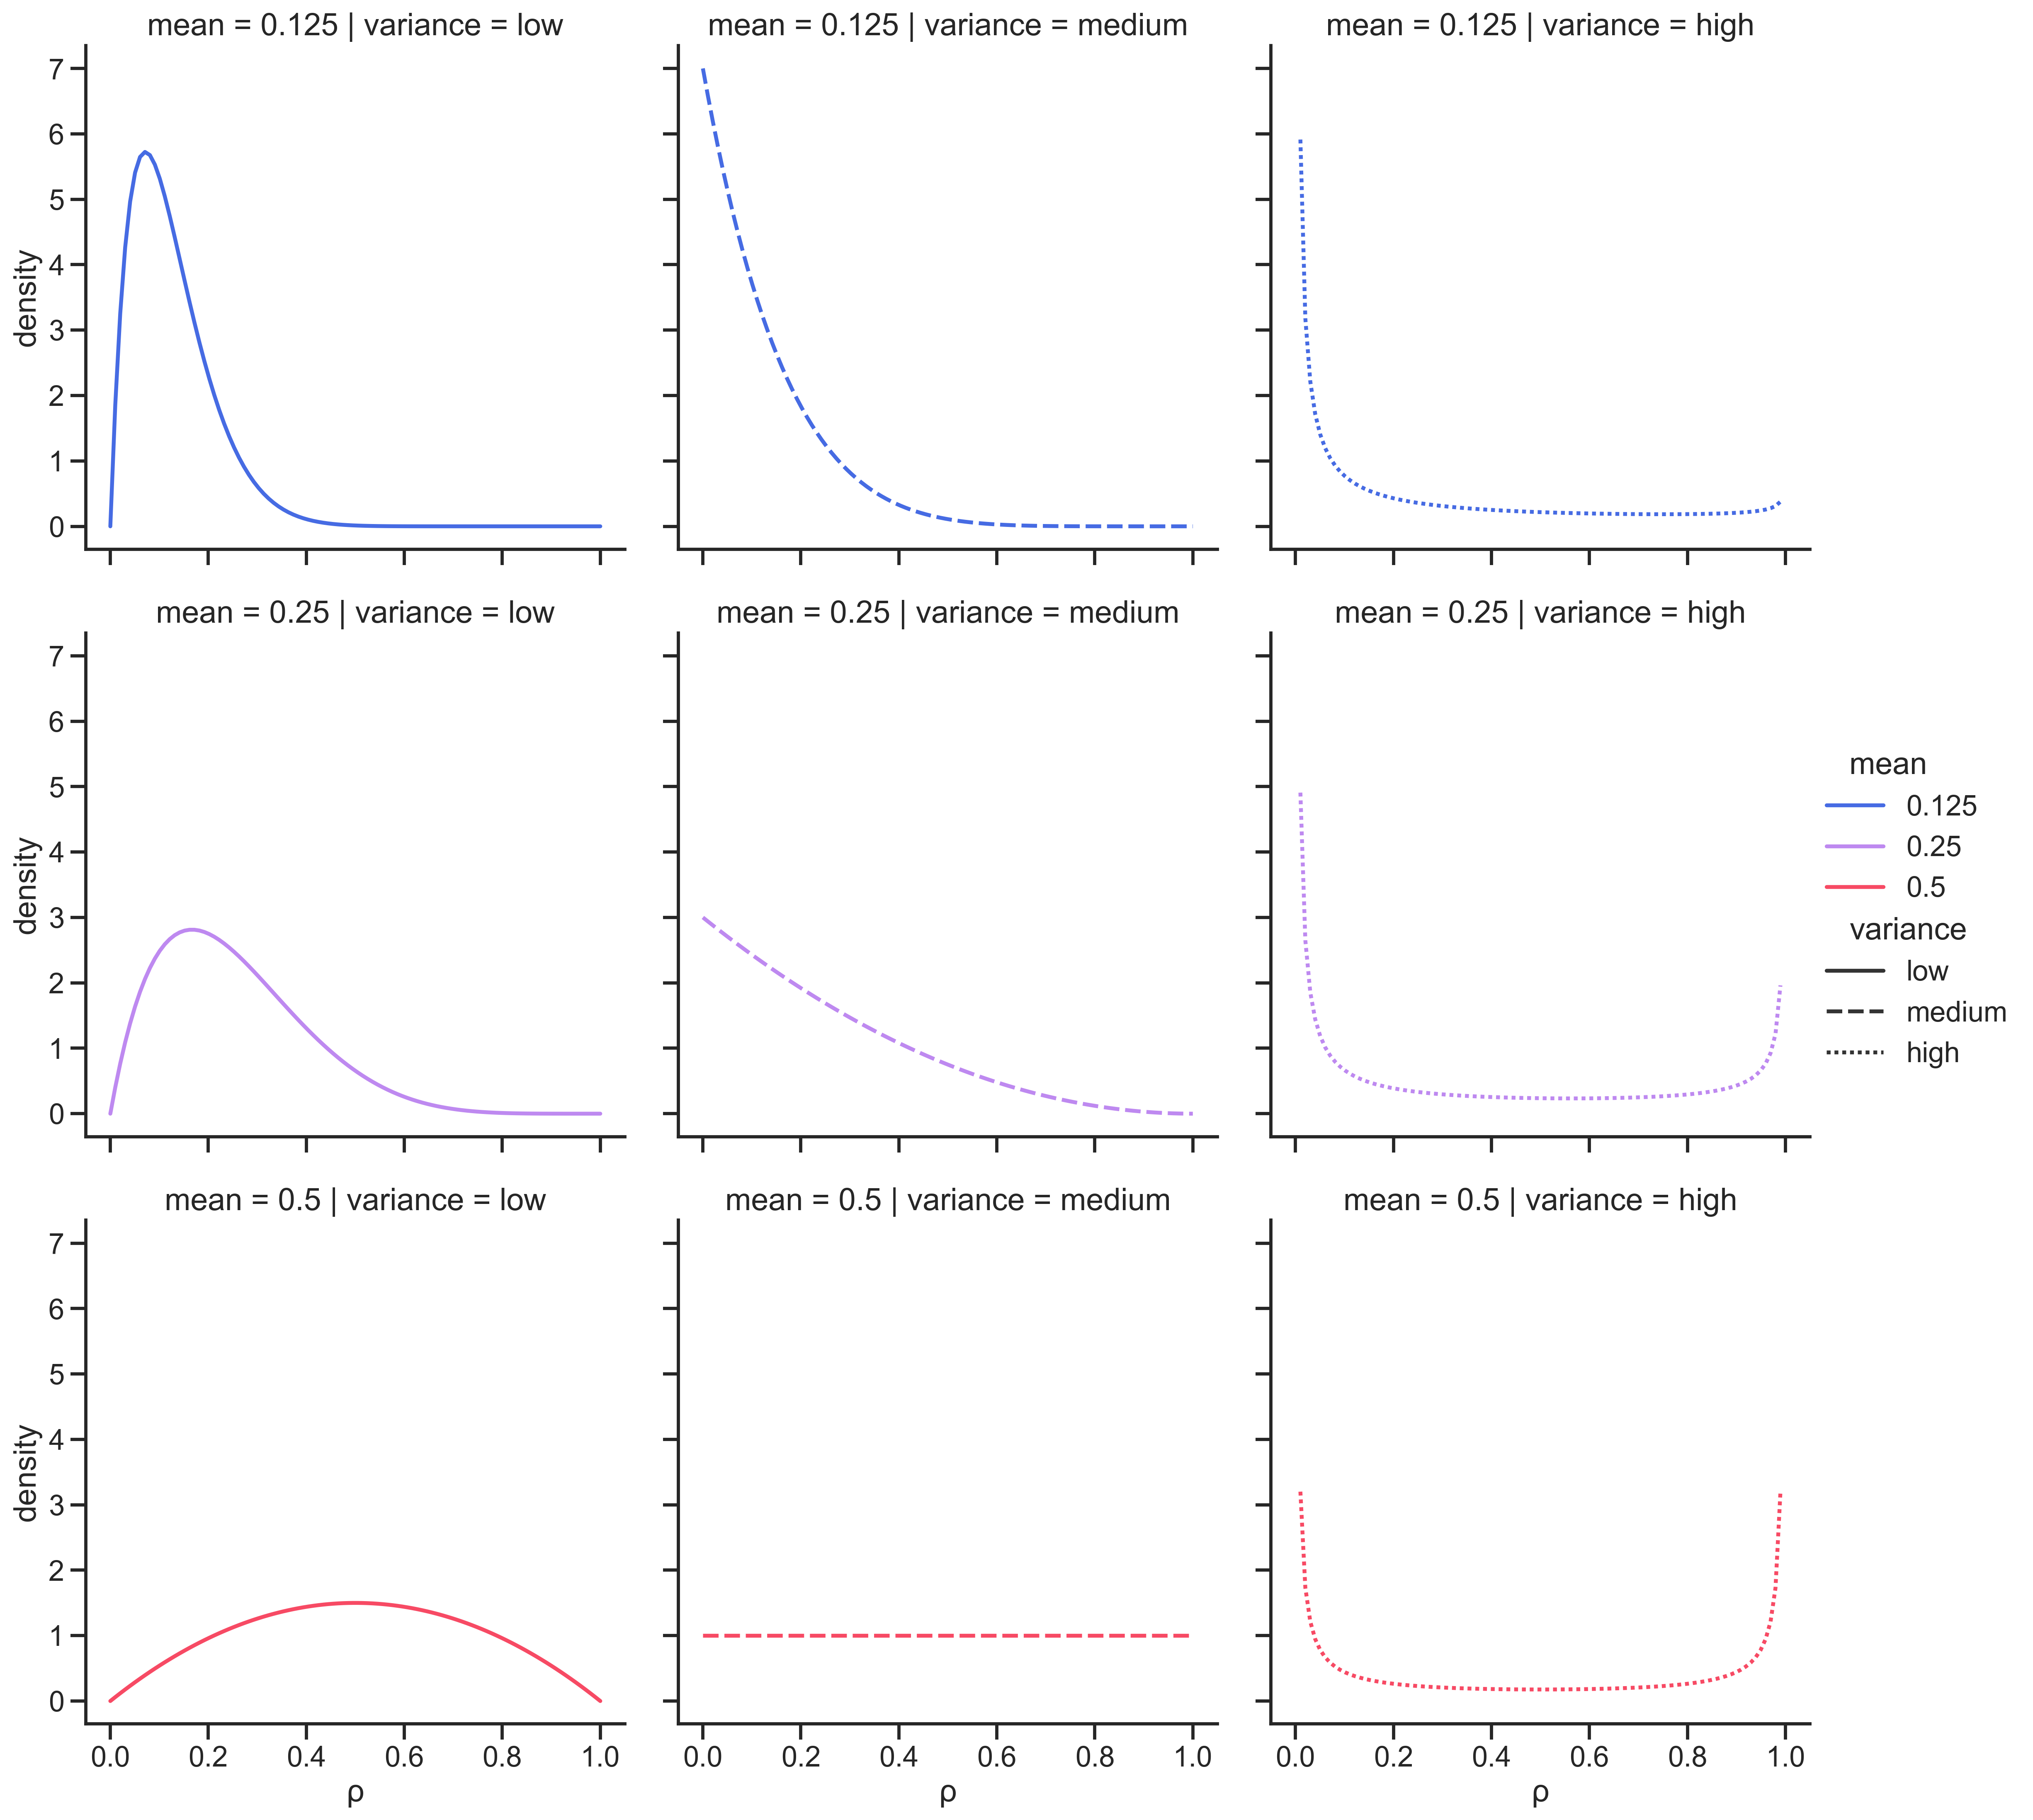
\includegraphics{images/risk_distributions.png}
\caption{\textbf{Risk distributions of the initial population:} the top
row shows distributions in which \textit{on average} 1/8th of the
population goes to the problem-place per week which increase in variance
from left to right. The second row shows the same with mean 1/4, and the
last row mean 1/2. We don't consider higher means -- if more than half
of the population spends time in the problem place per week, we start to
approach the homogeneous case.}
\end{figure}

Using this definition, we can compare scenarios where hot-spot spread
contributes \(1/4\), \(1/2\) or \(3/4\) of the expected disease spread
by varying \(\beta_c\) and \(\beta_p\), for the same \(R_0\).

Further, we can consider different shapes of the risk distribution
\(\mathrm{P}\).

In particular, we use nine different Beta distributions to consider
\(\mathrm{P}\)s with low, medium and high variability; and low (1/8),
medium (1/4), and high (1/4) means. These are shown in detail in {[}Beta
Distributions Figure{]}.

\subsubsection{Procedure}\label{procedure}

Our procedure is then the following:

We consider these three proportions of hot-spot spread; and within each,
nine distributions of risk taking; then we run simulations for values of
\(R_0\) ranging from 0 to 8 and compare the outcomes of the outbreaks to
those of a similar setup with no risk taking (the homogeneous case).

\subsection{2.3 Other Models}\label{other-models}

To aid in investigating the dynamics of the model in certain cases, we
consider and analytically analyze the following additional models.

\subsubsection{Branching process model}\label{branching-process-model}

When the number of infected agents is small; we use a branching process
model.

{[}this is developed more in the text{]}

\subsubsection{2.1.3 Integrodifferential
model}\label{integrodifferential-model}

Conversely, when the number of infected agents is large (either N is
very large or the number of infected agents is just large relative to
N), we consider the following integrodifferential equations:

\[
\begin{aligned}
\frac{\partial S(\rho, t)}{\partial t} &=
    -\beta_c S(\rho, t) \int_{0}^1 I(u, t) du
    -\beta_r S(\rho, t) \rho \int_{0}^1 I(u, t) u du\\
\frac{\partial I(\rho, t)}{\partial t} &=
    \beta_c S(\rho, t) \int_{0}^1 I(u, t) du
    + \beta_r S(\rho, t) \rho \int_{0}^1 I(u, t) u du - \gamma I(p, t)
\end{aligned}
\]

We analyze these equations and find several useful analytic results
which help to understand the general or expected dynamics of the system;
especially when N is large.

\subsubsection{2.1.4 Difference model}\label{difference-model}

Finally, to diagnose differences between the integrodifferential model
and the agent-based model we consider a difference equation model which
combines the deterministic behavior of the former with the discrete time
steps of the latter.

\subsection{3. Results}\label{results}

\subsubsection{3.1 Extinction Probability}\label{extinction-probability}

\paragraph{Homogeneous case}\label{homogeneous-case}

\begin{figure}
\centering
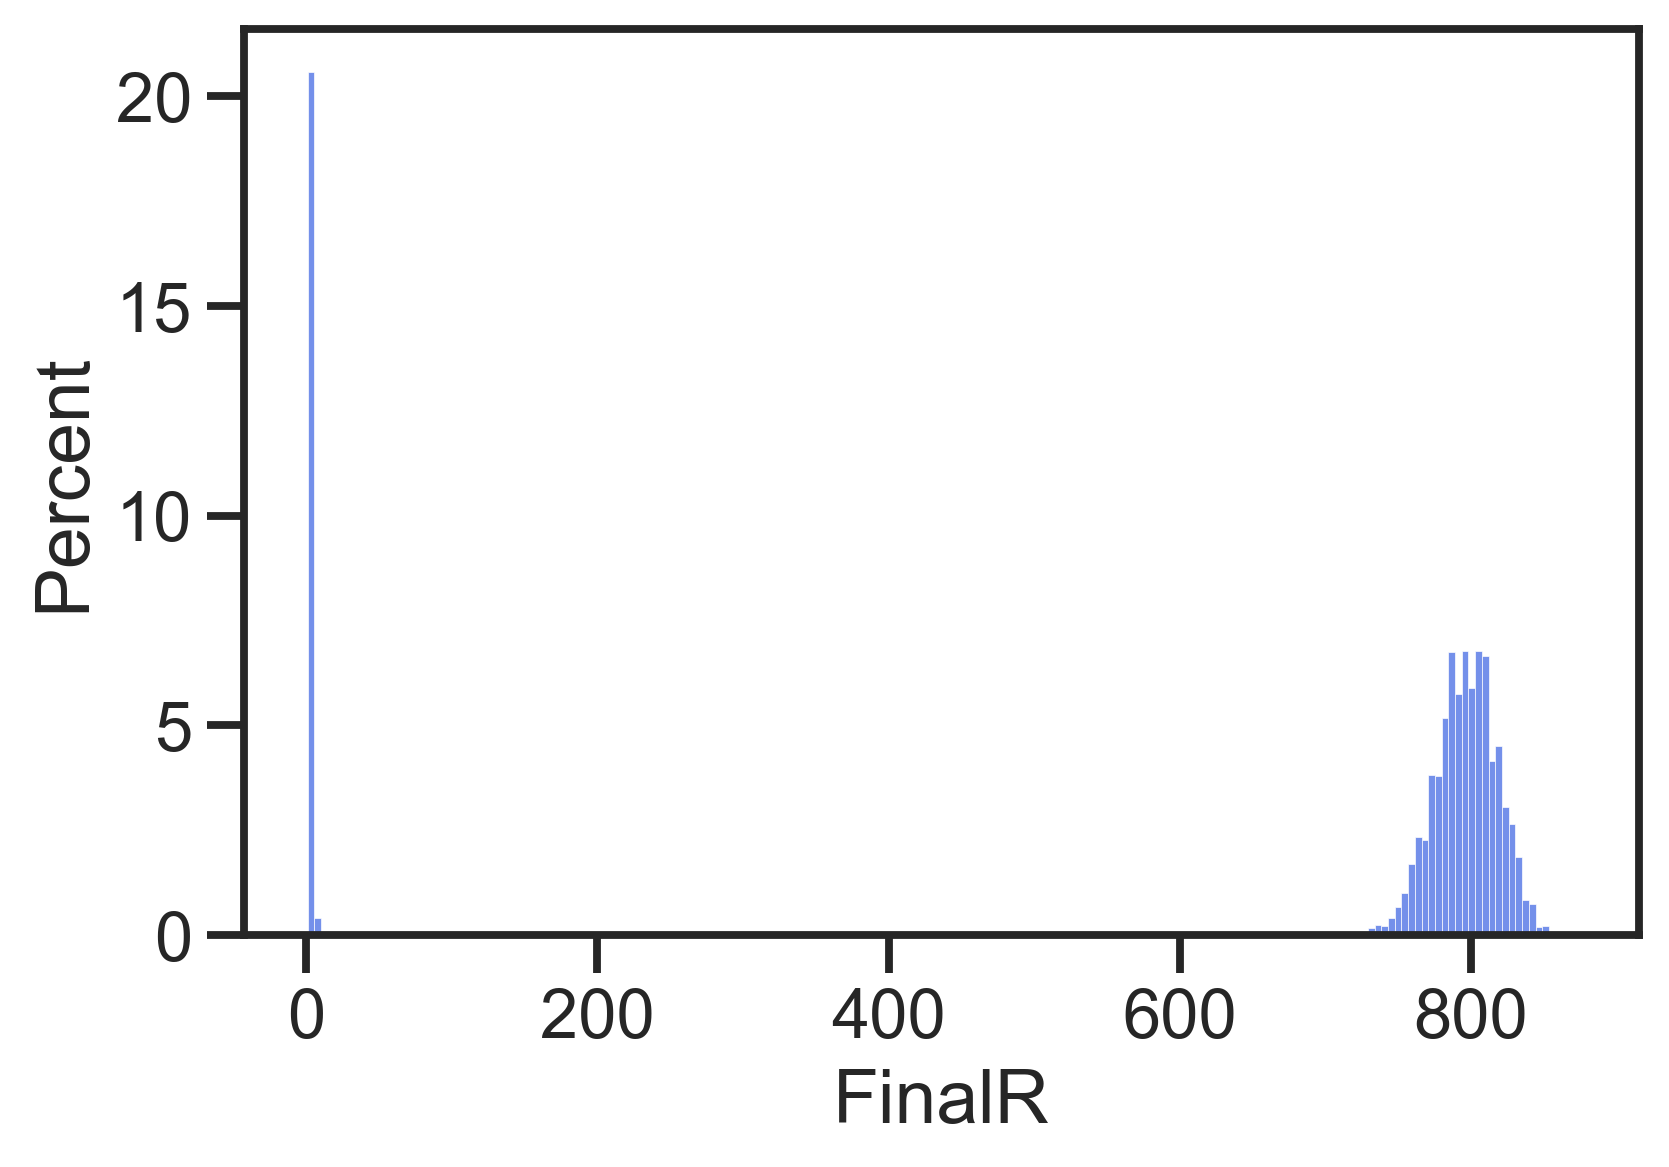
\includegraphics[width=0.5\textwidth,height=\textheight]{images/R2_histogram.png}
\caption{Histogram for homogeneous cases}
\end{figure}

\begin{figure}
\centering
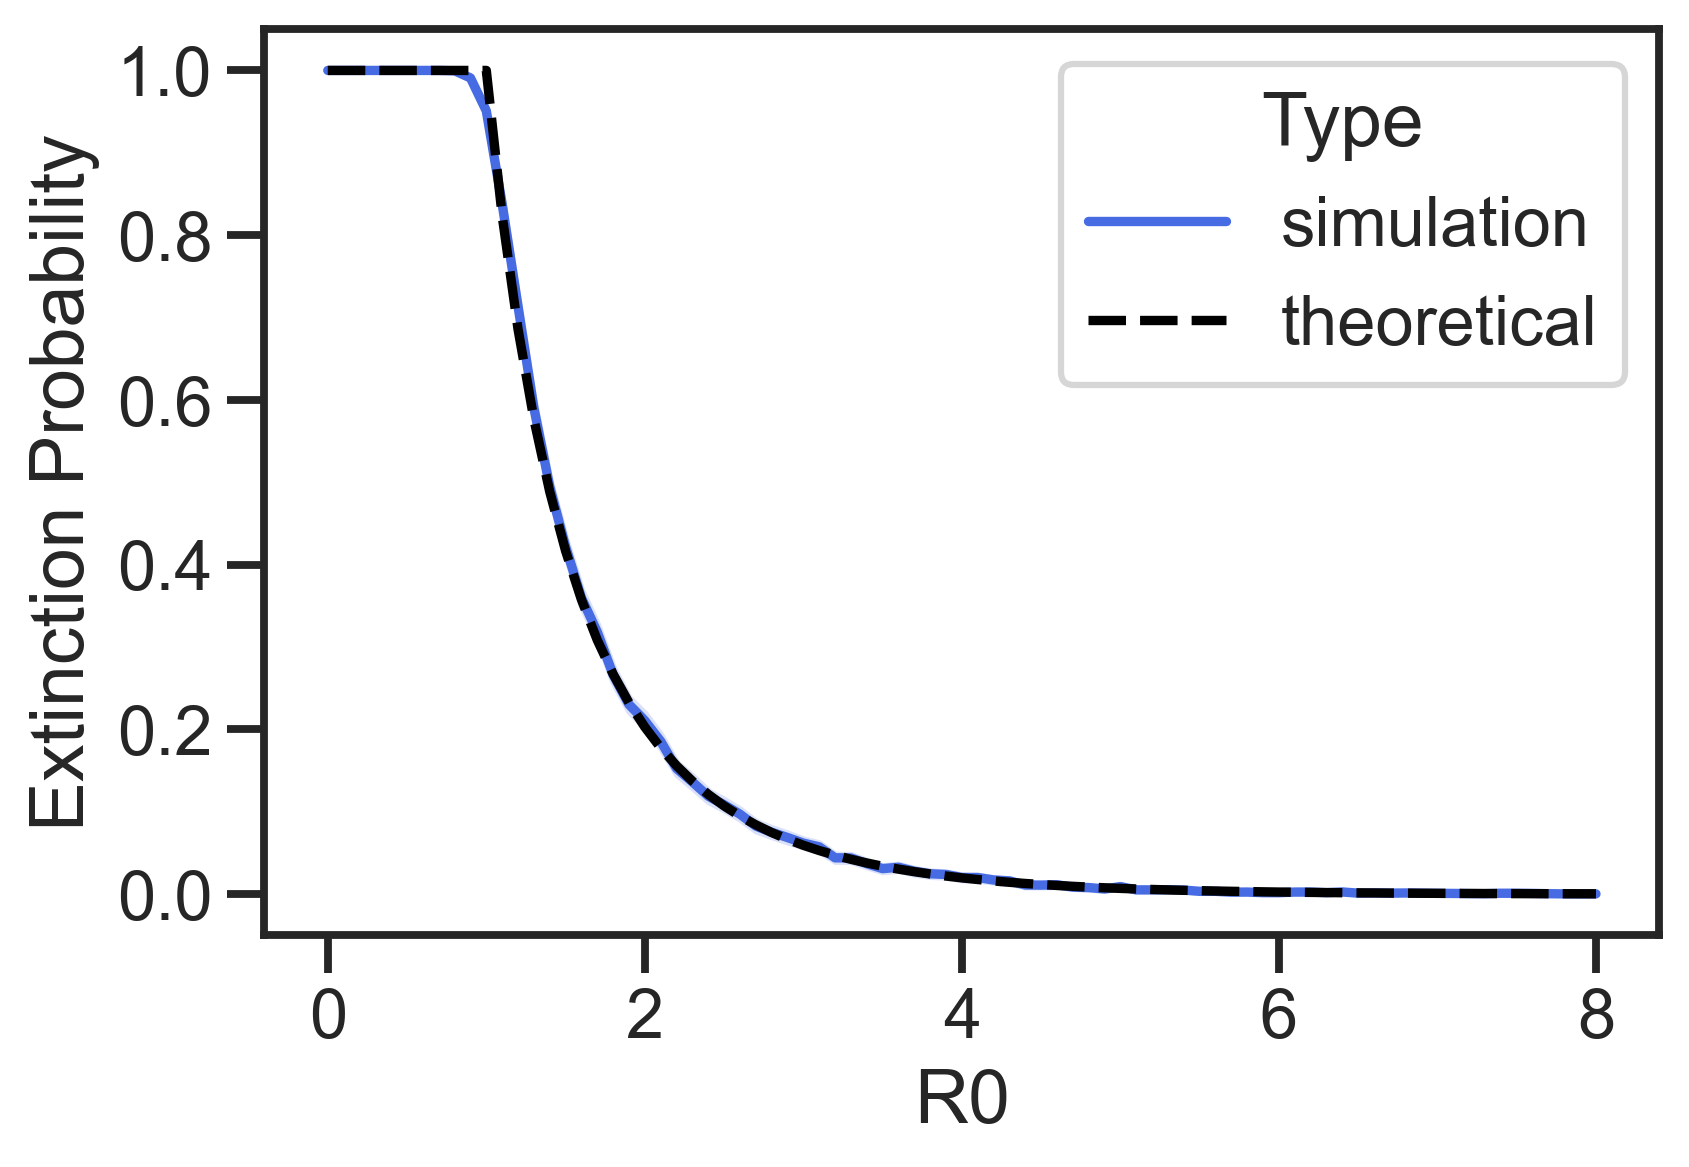
\includegraphics[width=0.5\textwidth,height=\textheight]{images/R2_extinction.png}
\caption{Figure that compares predicted extinction probability to
actual, for homogeneous case}
\end{figure}

Given a disease with \(\mathcal{R}_0\) of 2, the standard SIR model
predicts an outbreak to infect 79.681\% of the population before running
its course. When we simulate such an outbreak in a population of 1,000,
we see outbreaks of about this size, but we also see some number of
simulations in which there's no large outbreak at all.\textbackslash{}

We can predict the probability of a large vs small outbreak with
reasonable accuracy by replacing the outbreak scenario with a similarly
parameterized \textit{branching process}, and then asking how likely
this branching process is to go \textit{extinct}. This probability
\(\tau\) is a function of \(p(n)\) -- the probability of one individual
infecting \(n\) individuals before recovering. We make the simplifying
assumptions that: every infected individual can simultaneously go on to
infect \(N\) more individuals; essentially:

\begin{enumerate}
\def\labelenumi{\arabic{enumi}.}
\tightlist
\item
  every infected agent can go on to infect up to \(N\) more individuals
  (rather than N - (I + R)), and
\item
  secondary infections from multiple agents are independent (rather than
  considering how they are all infecting a shared population).
\end{enumerate}

Then under these assumptions, the extinction probability \(\tau\) obeys:

\[\tau = p(0) + p(1)\tau + p(2)\tau^2 + \ldots\]

In the approximation, \(p(n)\) is exactly the probability mass function
of a Binomial distribution with parameters
\(p=1 - (1 - \beta_c)^\gamma\) and \(N\), so the RHS of the equation
above is the generating function of the binomial distribution, which
gives:

\[\tau = (\tau (1 - (1 - \beta_c)^\gamma) + (1 - \beta_c)^\gamma)^N\]

This allows us to quite accurately predict the probability of a large
outbreak for any value of \(\mathcal{R}_0\) and compare to the simulated
results. We show this in {[}the figure above{]}.

\paragraph{Hotspot case}\label{hotspot-case}

\begin{figure}
\centering
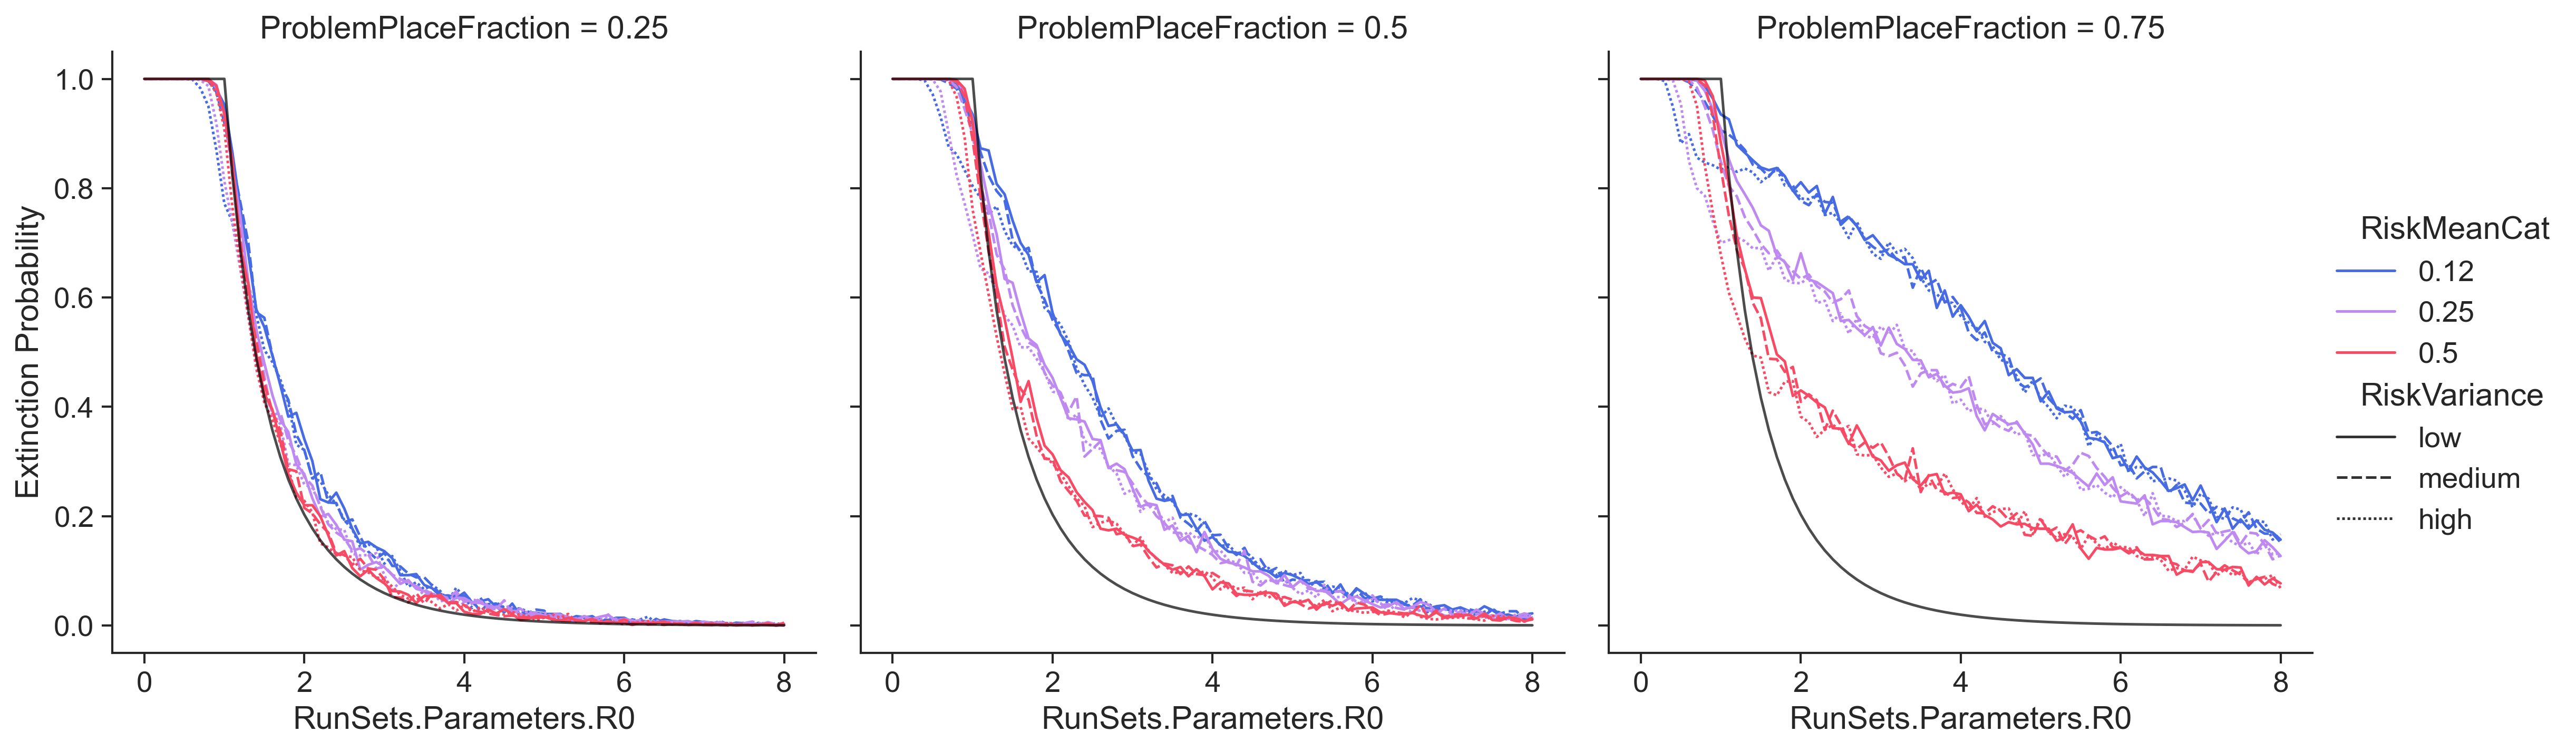
\includegraphics{images/extinction.png}
\caption{\textbf{Simulated extinction probabilities} Panels from left to
right show 25\%, 50\%, and 75\% of spread due to hot spot dynamics. Each
curve is extinction probability as \(R_0\) ranges from 0 to 8. Black
lines show extinction probability of the homogeneous (hot spot weight =
0\%) case for comparision.}
\end{figure}

\begin{figure}
\centering
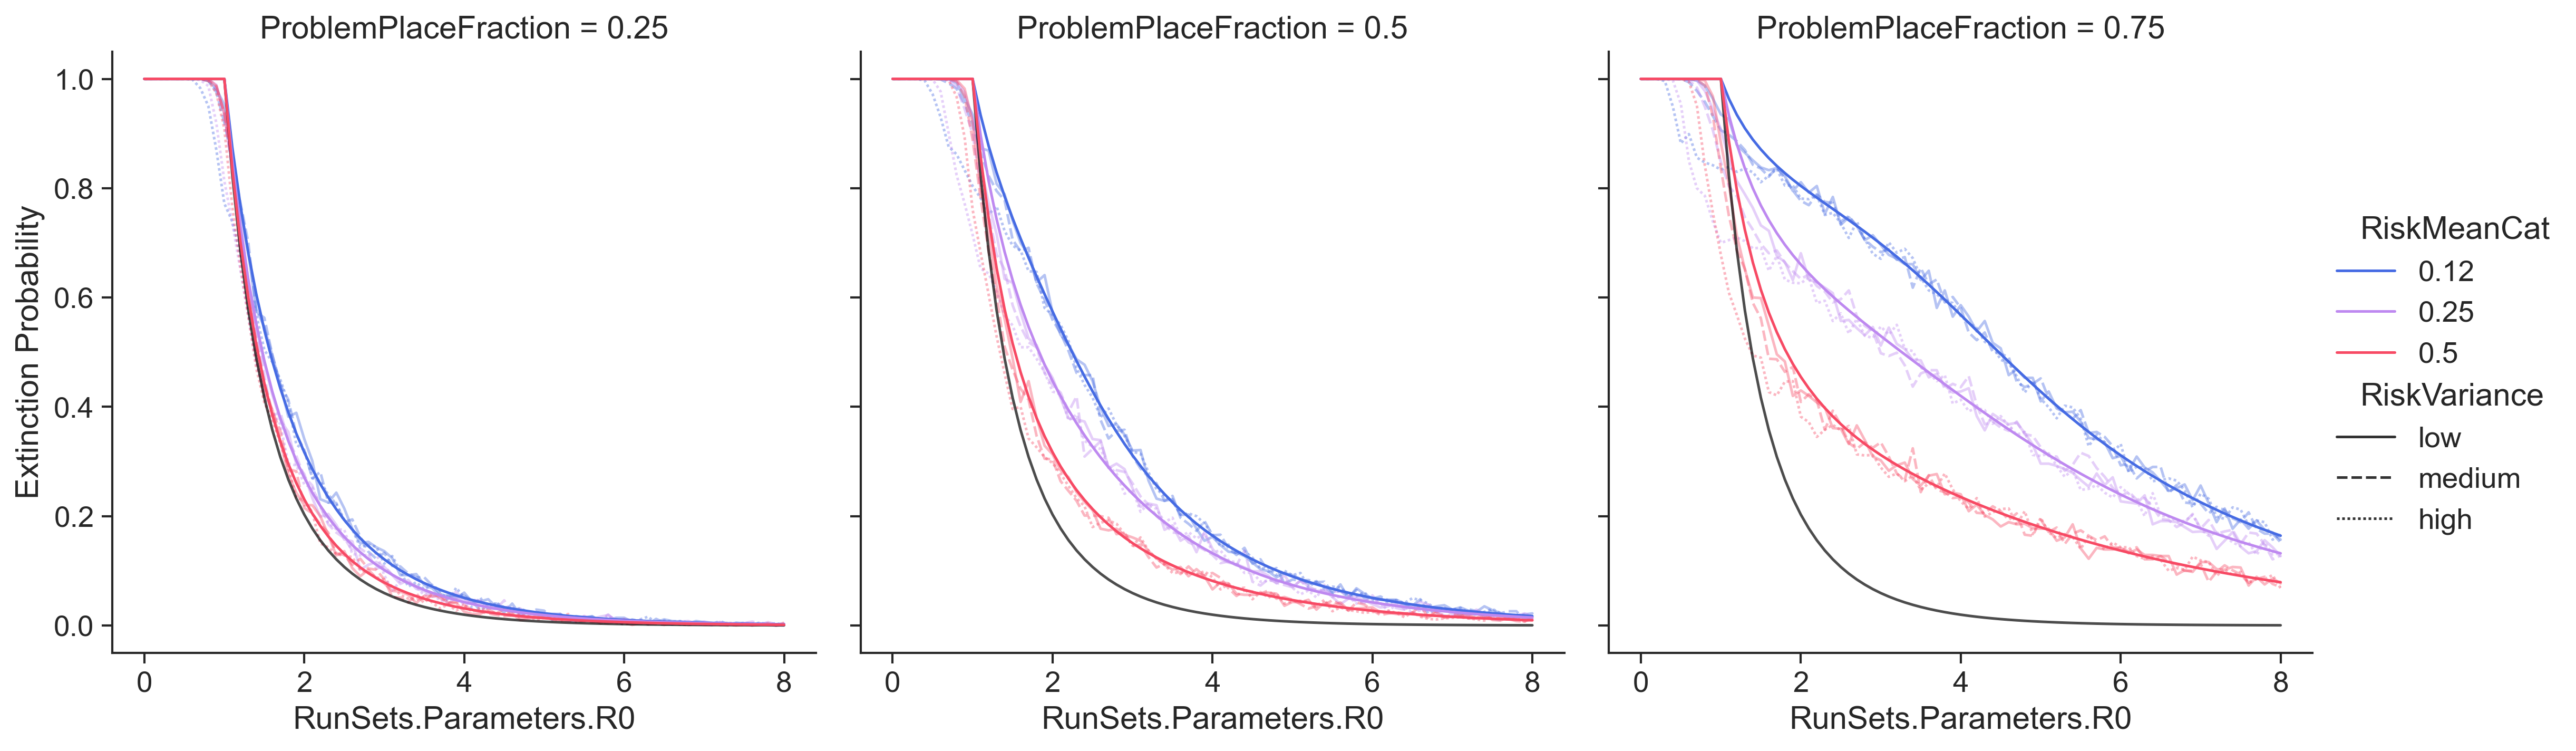
\includegraphics{images/extinction_theoretical.png}
\caption{\textbf{Similated vs theoretical extinction probabilities}}
\end{figure}

Now we consider the extinction probabilities observed in the agent-based
simulation, shown in {[}the figure above{]}. These deviate noticeably
from the homogeneous case even when controlling for \(R_0\).
Interestingly, the mean of the risk taking distribution \(\bar\rho\)
(line color) appears to play a large factor; while the skew of the risk
taking distribution (line dash style) plays apparently little or no
role.

We find that a similar branching process approximation helps explain
these findings. To the assumptions (1.) and (2.) above, we now add the
following:

\begin{enumerate}
\def\labelenumi{\arabic{enumi}.}
\setcounter{enumi}{2}
\tightlist
\item
  We now want \(E[\tau]\) -- the \emph{expected} extinction probability
  taking into account that the risk taking \(\rho\) of all individuals
  are drawn i.i.d. from the same distribution.
\end{enumerate}

Over the course of their infection, infected individual \(i\) with
riskyness \(\rho_i\) infects susceptible individual \(j\) (riskyness
\(\rho_j\)) through community spread with probability \(\beta_c\), or
through hot spot spread with probability \(\rho_i \rho_j \beta_r\) (they
must both go to the hot spot). Combined, this is:

\[\beta_c + (1 - \beta_c)(\rho_i \rho_j \beta_r)\]

In expectation, since the \(\rho\) are drawn iid, this is:

\[\beta_c + (1 - \beta_c)(\bar\rho^2 \beta_r) = \beta_{\text{effective}}\]

And as before, \(p(n)\) is a Binomial probability mass; here with
\(\beta_{\text{effective}}\) and \(N\).

Finally, we make one more simplifying assumption:

\begin{enumerate}
\def\labelenumi{\arabic{enumi}.}
\setcounter{enumi}{3}
\tightlist
\item
  Individuals infected after the first have expected riskyness
  \(\bar\rho\).
\end{enumerate}

This neglects the fact that individuals infected after the first should
tend to have a higher riskyness -- but this is necessary to use a
branching process model.

With these assumptions, following a similar approach (see appendix) to
above we find that:

\[E[\tau] = \bar\rho [(1 - \bar\rho \beta_r)(1 - \beta_c) + 
                (1 - (1 - \bar\rho \beta_r)(1 - \beta_c) \tau]^N + 
   (1 - \bar\rho)[(1 - \beta_c) + \beta_c \tau]^N\\\]

These predictions are shown in {[}figure above{]} compared to the
simulated results from {[}fig:extinction\_results{]}, showing great
agreement. Both predict that nearly across the board disease extinction
is more probable than in the homogeneous case. In keeping with
{[}superspreader papers{]}, spread is concentrated in some individuals
more than others. When these individuals are among the first infected,
the outbreak may be more explosive; but conversely there the initial
infection may not find a superspreader and even for very high
\(\mathcal{R}_0\) the disease peters out. Conversely, we see some
possibility of an outbreak for \(\mathcal{R}_0 < 1\) -- a probabilistic
impossibility in the homogeneous scenario. In this case, what we're
seeing is a small outbreak localized among the high risk-taking
subpopulation -- if we looked at this subpopulation alone there is
\(\mathcal{R}_0 > 1\).

Additionally, the fact of this model agreement alone has interesting
implications. It suggests that the factors we're leaving out -- (a) the
differences in the shapes of distributions beyond their mean; and (b)
the accelerative effect as later generations of infected agents have
generally higher riskyness -- only become significant later on, at a
point in which outbreak extinction has already become vanishingly
unlikely.

\subsubsection{3.2 Max I, Total R}\label{max-i-total-r}

\begin{figure}
\centering
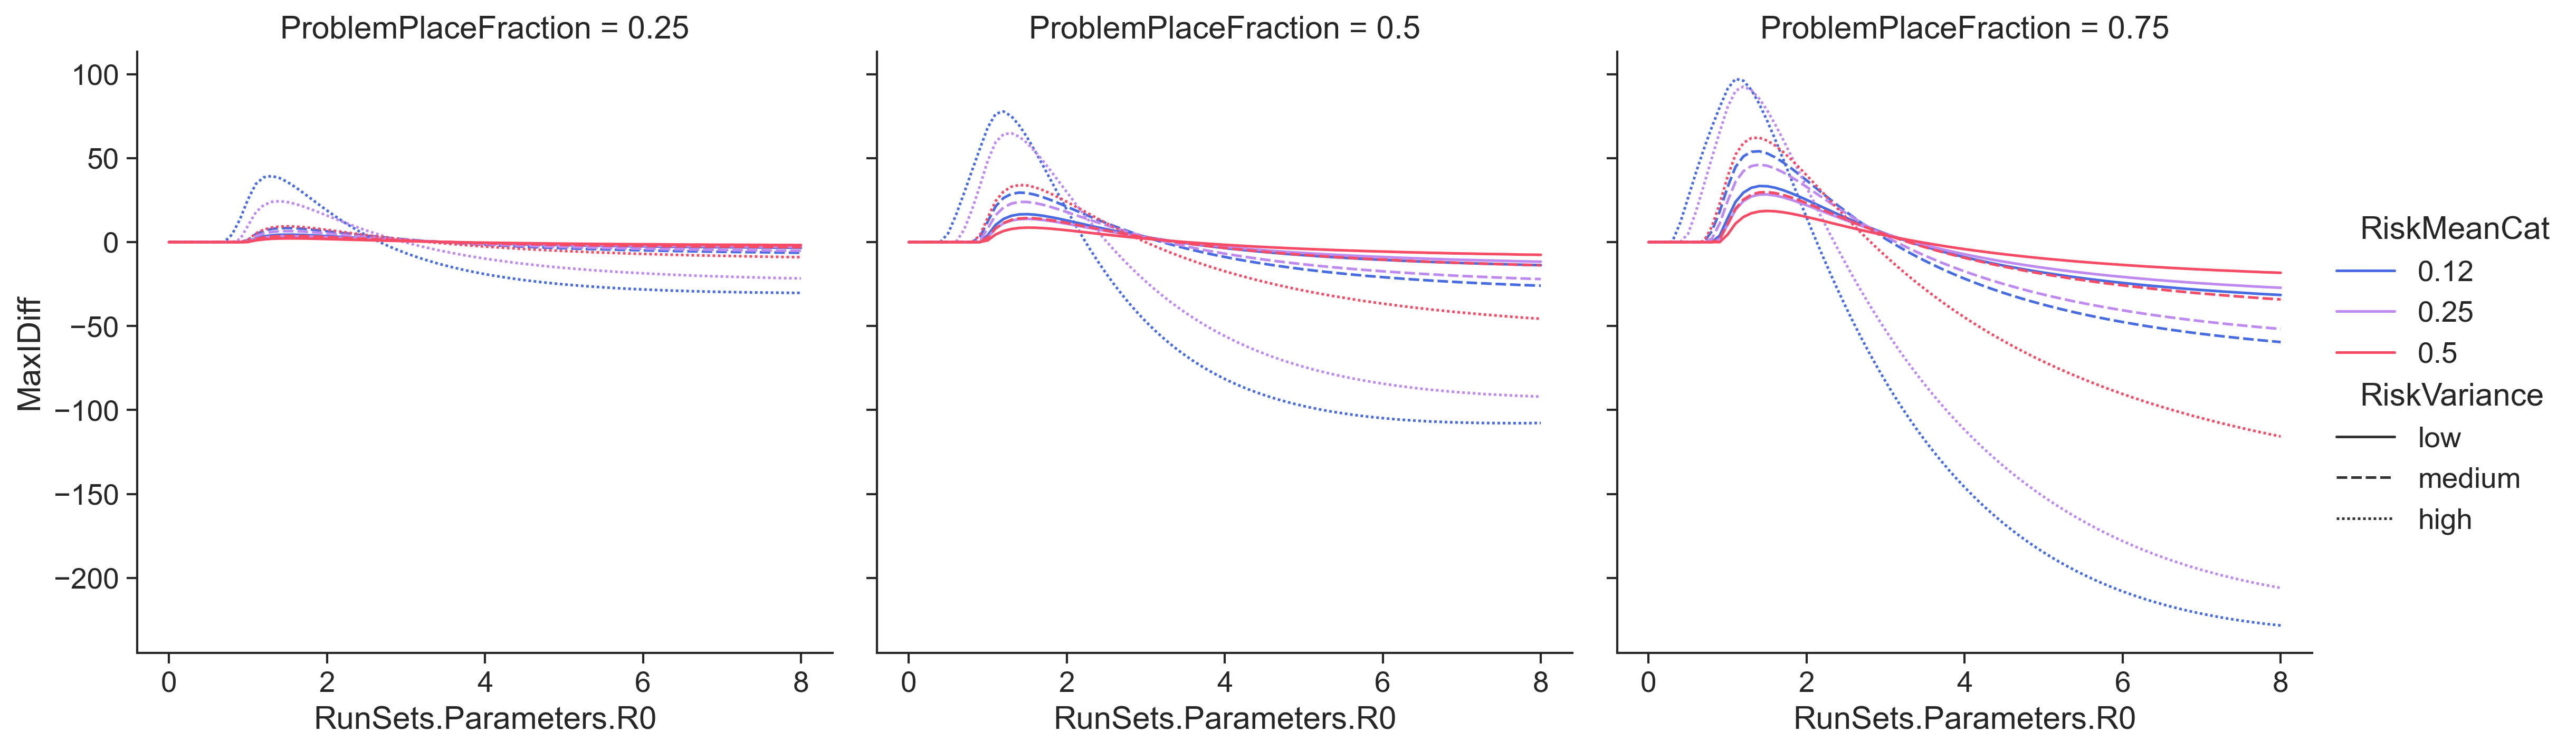
\includegraphics{images/MaxI.png}
\caption{Max I}
\end{figure}

\begin{figure}
\centering
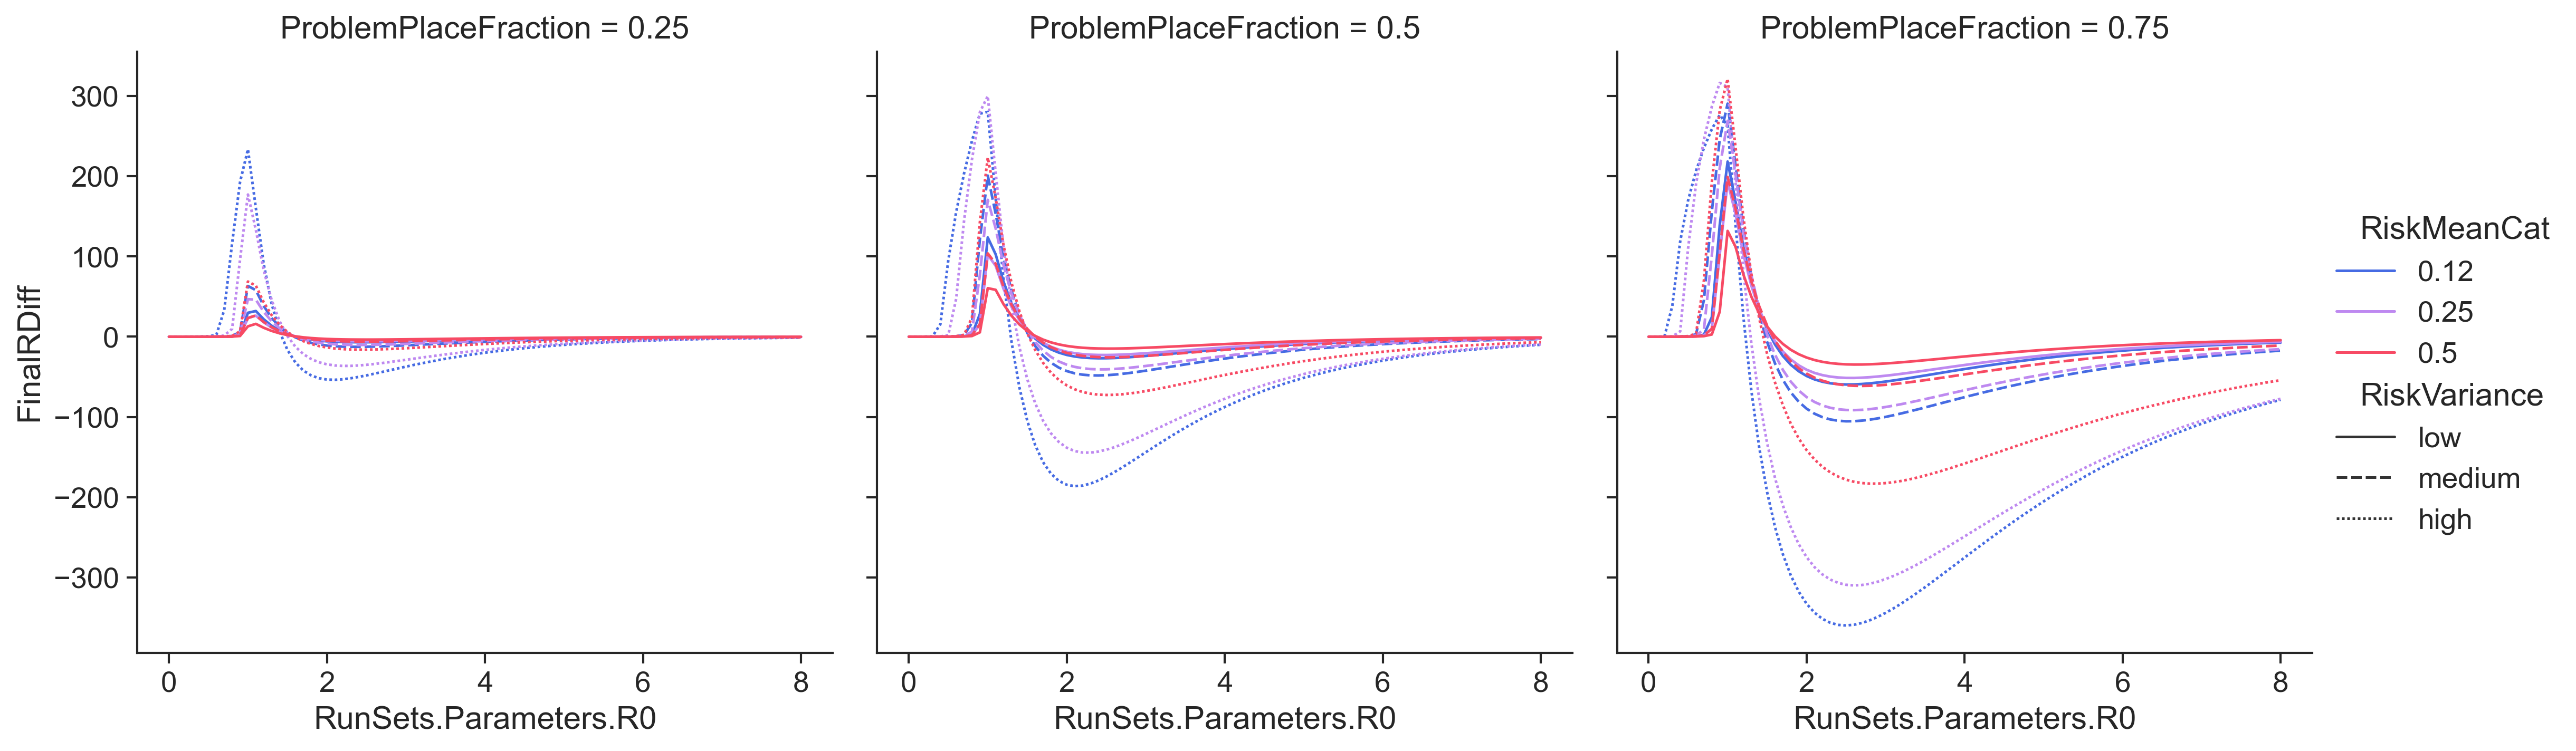
\includegraphics{images/FinalR.png}
\caption{Final R}
\end{figure}

Next we look at only those scenarios in which an outbreak occurs and ask
how problem place dynamics affect the size and severity of the outbreak.
We consider Max I -- the peak number of infected individuals -- and
Final R -- the total number individuals infected (and recovered) over
the entire course of the outbreak. Similar to {[}Extinction Probability
Section{]} we fix a value of \(\mathcal{R}_0\), then for the risk
distributions discussed in {[}Intro Section{]} we vary the contribution
of problem place spread and observe the effects. This is shown in
{[}fig:outbreak\_results{]}.

\begin{itemize}
\tightlist
\item
  For very low \(\mathcal{R}_0\) (below about 1.5), we see significantly
  larger outbreaks. (Here, as above, an outbreak is ocurring mostly just
  among the subpopulation with very large riskyness.)
\item
  For moderate \(\mathcal{R}_0\) (1.5 to somewhere between 2.0 and 3.0),
  we see a mixed result: outbreaks have a higher number of infections at
  their peak, but overall affect fewer individuals.
\item
  And finally, for high \(\mathcal{R}_0\) (somewhere above 2.0 to 3.0)
  outbreaks are less severe both in the total and the peak number of
  infections.
\end{itemize}

\subsubsection{3.3 Disease Evolution}\label{disease-evolution}

Finally, to explain the findings of {[}3.2{]} we analyze how the disease
plays out over time during an outbreak. Here the differential equation
model is useful.

In the analysis section we show that the basic reproduction number
\(R(t)\) is given by:

\textbf{TODO: Remake this figure. can convey much more information if
this is nicely done.}

\begin{figure}
\centering
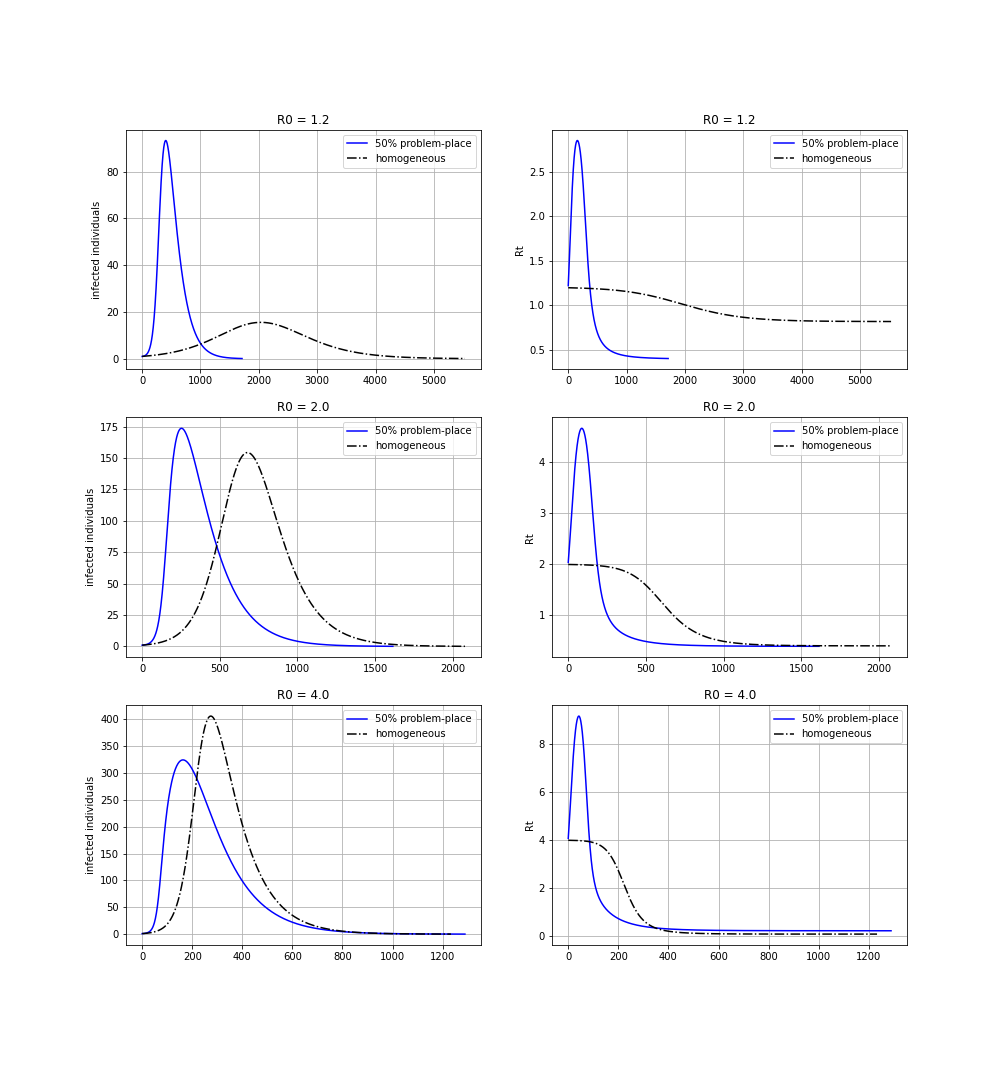
\includegraphics{images/dynamics_comparison.png}
\caption{Dynamics Comparison}
\end{figure}

In {[}dynamics figure{]} we plot the dynamics of several outbreaks over
time. We see all three scenarios: a much larger wave of infections for
low \(R0\), one with a narrower but slightly higher peak for moderate
\(R0\), and a lower and smaller wave entirely for large \(R0\). The peak
of the outbreak occurs significantly earlier in all three cases.

Comparing \(R(t)\) helps explain these differences. In the homogeneous
case, \(Rt\) decreases monotonically. In the hot spot model, \(Rt\)
increases initially, peaks sharply, then falls off; causing the entire
outbreak to accelerate.

This is evident in {[}figure above{]}, and can be shown universally.
First, recall the equation for effective \(Rt\):

\[R(t) = \frac{\bar S}{\gamma} \left( \beta_c + \beta_r \bar \rho_S \bar \rho_I \right)\]

\(Rt\) has similar form to the homogeneous
\(Rt = \frac{S}{\gamma} \beta\); except \(\beta\) is replaced by
\(\left( \beta_c + \beta_r \bar \rho_S \bar \rho_I \right)\) - which we
could call ``effective beta'' and which is governed by \(\bar\rho_I\)
and \(\bar\rho_S\).

\textbf{Claim 1: \(\bar\rho_S\) decays monotonically in proportion to
\(\beta_r\), the total infected population size, \(\bar\rho_I\) and the
variance of \(\rho_S\).}

\textbf{Claim 2: \(\bar{\rho_I}\) moves towards a fixed value between
\(\bar\rho_S\) and
\(\bar\rho_S + \frac{\text{Var}(\rho_S)}{\bar\rho_S}\).}

These claims follow from the following results, which are derived in the
appendix:

\[
\frac{d}{dt}\bar\rho_S = -\beta_r \bar I \bar\rho_I \text{Var}(\rho_s)
\]

\[
\frac{d}{dt}\bar\rho_I
= \bar S \left[
    \beta_c (\bar\rho_S - \bar\rho_I)
    + \beta_r \bar\rho_S \bar\rho_I((\bar\rho_S + \frac{\text{Var}(\rho_S)}{\bar\rho_S})
        - \bar\rho_I))\right]
\]

(The latter equation contains the sum of two restorative forces: one
pushes \(\bar\rho_I\) towards \(\bar\rho_I\), and the other towards
\(\bar\rho_S + \frac{\text{Var}(\rho_S)}{\bar\rho_S}\). So there must be
some value in between towards which \(\bar\rho_I\) is forced, as
claimed.)

\subsection{4. Discussion}\label{discussion}

\emph{I wanted to get some feedback on this outline for the discussion
section before trying too hard to write everything out.}

(note to myself: hourglass back out)

Outline:

\begin{itemize}
\item
  review caveats and model assumptions (though I suppose that's covered
  in appendices A.5 and A.6)
\item
  discuss these ``gravity law of movement'' papers I've been reading;
  and use them to inform which distributions make the most sense
\item
  discuss laurant's papers about superspreading events
\item
  discuss dobromir's \& mark's paper about the more general case of risk
  structure
\item
  further work:

  \begin{itemize}
  \tightlist
  \item
    could look into the implications of this on intervention timing
    (could cite my other paper if it gets published in time??) (I did
    look into this briefly but it wasn't super interesting at first
    pass)
  \end{itemize}
\end{itemize}

\subsection{A. Appendix}\label{a.-appendix}

\begin{itemize}
\tightlist
\item
  A.1 branching process derivations
\item
  A.2 differential equations - moments
\item
  A.3 basic reproduction number
\item
  A.4 differential equations - mean riskyness results
\item
  A.5 choice of \(\gamma\) and \(N\)
\item
  A.6 model comparisons
\end{itemize}

\subsubsection{A.1 Disease Extinction}\label{a.1-disease-extinction}

Derivation of the branching process approximation:

\[E[\tau] = \bar\rho [(1 - \bar\rho \beta_r)(1 - \beta_c) + 
                (1 - (1 - \bar\rho \beta_r)(1 - \beta_c) \tau]^N + 
   (1 - \bar\rho)[(1 - \beta_c) + \beta_c \tau]^N\\\]

Here we show that we can apply the same branching process approximation
to the problem-place model to predict the probability of a large
outbreak under any set of parameters.

Let X be a random variable that represents the number of infections
caused by a single infected individual with riskyness \(\rho_i\) before
recovering, and let \(j = 1, \ldots, N\) index the susceptible
population so that \(\rho_j\) is the riskyness of individual \(j\).

Then
\[P(X = 0) = (1 - \rho_i) [ (1 - \beta_c)^N ] + \rho_i [ \prod_j (1 - (\beta_c + \beta_r \rho_j)) ]\]

By assumption riskyness for each individual is drawn independently from
one distribution, so in expectation (over riskyness values) this is:

\[
\begin{aligned}
E[P(X = 0)] &= E[(1 - \rho_i) [ (1 - \beta_c)^N ] + \rho_i [ \prod_j (1 - (\beta_c + \beta_r \rho_j)) ]]\\
&= (1 - E[\rho_i]) [ (1 - \beta_c)^N ] + E[\rho_i] [ \prod_j (1 - (\beta_c + \beta_r E[\rho_j])) ]]\\
&= (1 - \bar\rho) [ (1 - \beta_c)^N ] + \bar\rho [(1 - (\beta_c + \beta_r \bar\rho))^N ]\\
&= (1 - \bar\rho) B(\beta_c, N, 0) + \bar\rho B(\beta_c + \bar\rho \beta_r, N, 0)\\
\end{aligned}
\]

Where \(B(a, b, x)\) is the Binomial probability mass at x with
parameters a and b.

Similarly, \(E[P(X) = x]\) is given by

\[(1 - \bar\rho) B(\beta_c, N, x) + \bar\rho B(\beta_c + \bar\rho \beta_r, N, x)\]

So

\[
\begin{aligned}
G_X(s) &= P(X=0) + P(X=1)s + P(X=2)s^2 + \ldots\\
&= [\bar\rho B_1(0) + (1 - \bar\rho)B_2(0)] + [\bar\rho B_1(1) + (1 - \bar\rho)B_2(1)]s + [\bar\rho B_1(2) + (1 - \bar\rho)B_2(2)]s^2 + \ldots\\
&= \bar\rho G_{B_1}(s) + (1 - \bar\rho)G_{B_2}(s)\\
&= \bar\rho [(1 - \bar\rho \beta_r)(1 - \beta_c) + 
                (1 - (1 - \bar\rho \beta_r)(1 - \beta_c) s]^N + 
   (1 - \bar\rho)[(1 - \beta_c) + \beta_c s]^N\\
\tau &= \bar\rho [(1 - \bar\rho \beta_r)(1 - \beta_c) + 
                (1 - (1 - \bar\rho \beta_r)(1 - \beta_c) \tau]^N + 
   (1 - \bar\rho)[(1 - \beta_c) + \beta_c \tau]^N\\
\end{aligned}
\]

\subsubsection{A.2 Moment equations}\label{a.2-moment-equations}

Initial equations:

\[
\begin{aligned}
\frac{\partial S(\rho, t)}{\partial t} &=
    -\beta_c S(\rho, t) \int_{0}^1 I(u, t) du
    -\beta_r S(\rho, t) \rho \int_{0}^1 I(u, t) u du\\
\frac{\partial I(\rho, t)}{\partial t} &=
    \beta_c S(\rho, t) \int_{0}^1 I(u, t) du
    + \beta_r S(\rho, t) \rho \int_{0}^1 I(u, t) u du - \gamma I(p, t)
\end{aligned}
\]

For convenience, we introduce the following shorthands for the
``moments'' of \(I(\rho)\) and \(S(\rho)\):

\[
\begin{aligned}
\bar S &:= \int_{0}^{1} S(\rho) d\rho
    & \bar I &:= \int_{0}^{1} I(\rho) d\rho\\
\hat S &:= \int_{0}^{1} S(\rho) \rho d\rho
    & \hat I &:= \int_{0}^{1} I(\rho) \rho d\rho\\
\hat{\hat{ S}} &:= \int_{0}^{1} S(\rho) \rho^2 d\rho
    & \hat{\hat{ I}} &:= \int_{0}^{1} I(\rho) \rho^2 d\rho\\
\vdots & & \vdots \\
\overset{(n)}{S} &:= \int_{0}^{1} S(\rho) \rho^n d\rho
    & \overset{(n)}{I} &:= \int_{0}^{1} I(\rho) \rho^n d\rho\\
\end{aligned}
\]

Now we can more concicely write the initial equations:

\[
\begin{aligned}
\frac{\partial S(\rho, t)}{\partial t} &=
    -\beta_c S(\rho, t) \bar I
    -\beta_r S(\rho, t) \rho \hat I\\
\frac{\partial I(\rho, t)}{\partial t} &=
    \beta_c S(\rho, t) \bar I
    + \beta_r S(\rho, t) \rho \hat I - \gamma I(p, t)
\end{aligned}
\]

Finally, notice that \(S(\rho)\) and \(I(\rho)\) are defined over
\(\rho \in [0, 1]\), and that these give the population at a given risk
level. We can equivalently think of how risk is distributed over the S
and I populations:

We introduce \(\rho_S\) and \(\rho_I\): these are random variables drawn
from the distributions of risk in the S and I populations, respectively.

The means of these variables are:

\[
\begin{aligned}
\bar\rho_S
&= \frac{\int_{0}^{1} S(\rho) \rho d\rho}{\int_{0}^{1} S(\rho) d\rho}
= \frac{\hat S}{\bar S}\\
\bar\rho_I
&= \frac{\int_{0}^{1} I(\rho) \rho d\rho}{\int_{0}^{1} I(\rho) d\rho}
= \frac{\hat I}{\bar I}\\
\end{aligned}
\]

(This is just setting up interpretable variables for the terms
\(\frac{\hat S}{\bar S}\) and \(\frac{\hat I}{\bar I}\), which start to
pop up in a bunch of places.)

First we have a general result relating the ``moments'' of S and I.

Suppose we want to know how the total susceptible population is
changing. We can integrate \(\frac{\partial S}{\partial t}\) over
\(\rho\):

\[
\begin{aligned}
\frac{d \bar{S}}{dt} = \int_{0}^{1} \frac{\partial S(\rho)}{\partial t} d\rho
&= \int_{0}^{1} (-\beta_c S(\rho) \bar I - \beta_r S(\rho) \rho \hat I) d\rho  \\
&= -\beta_c (\int_{0}^{1} S(\rho) d\rho) \bar I
    - \beta_r (\int_{0}^{1} S(\rho) \rho d\rho) \hat I\\
&= -\beta_c \bar S \bar I - \beta_r \hat S \hat I
\end{aligned}
\]

Similary, we can find that:

\[\frac{d \bar{I}}{dt} = \int_{0}^{1} \frac{\partial I(\rho)}{\partial t} d\rho
= \beta_c \bar S \bar I + \beta_r \hat S \hat I - \gamma \bar I\]

If we want to see how the first moments are changing, we follow a
similar method: \[
\begin{aligned}
\frac{d \hat{S}}{dt} = \int_{0}^{1} \frac{\partial S(\rho)}{\partial t} \rho d\rho
&= \int_{0}^{1} (-\beta_c S(\rho) \bar I - \beta_r S(\rho) \rho \hat I) \rho d\rho  \\
&= -\beta_c (\int_{0}^{1} S(\rho) \rho d\rho) \bar I
    - \beta_r (\int_{0}^{1} S(\rho) \rho^2 d\rho) \hat I\\
&= -\beta_c \hat S \bar I - \beta_r \hat{\hat{ S}} \hat I
\end{aligned}
\]

And for any general moment:

\[
\begin{aligned}
\frac{d \overset{(n)}{S} }{dt} &=
    -\beta_c \overset{(n)}{S} \bar I
    -\beta_r \overset{(n+1)}{S} \hat I \\
\frac{d \overset{(n)}{I}}{dt} &=
    \beta_c \overset{(n)}{S} \bar I
    + \beta_r \overset{(n+1)}{S} \hat I - \gamma \overset{(n)}{I}
\end{aligned}
\]

\subsubsection{A.3 Basic Reproduction
Number}\label{a.3-basic-reproduction-number}

In the homogeneous SIR model, the basic reproduction number (number of
secondary infections per infection) is:

\[\mathcal{R}_t = \frac{S\beta}{\gamma}\]

In this model, we can derive a similar form for the expected number of
secondary infections per infection by dividing \(\frac{d \bar S}{dt}\)
by \(\hat I\) (current number of infected individuals) then multiplying
by the mean duration of an infection \(\frac{1}{\gamma}\). \[
\begin{aligned}
\mathcal{R}_t &= -\frac{d\bar S}{dt} \frac{1}{\gamma \bar I} \\
    &= \frac{1}{\gamma} \beta_c \bar S \frac{\bar I}{\bar I}
        + \frac{1}{\gamma} \beta_r \hat S \frac{\hat I}{\bar I}\\
    &= \frac{1}{\gamma} \bar S\left( \beta_c
        + \beta_r \frac{\hat S}{\bar S} \frac{\hat I}{\bar I} \right)\\
    &= \frac{1}{\gamma} \bar S\left( \beta_c
        + \beta_r \bar \rho_S \bar \rho_I \right)\\
\end{aligned}
\]

This gives a nicely analogous result, where the homogenous \(\beta\) is
replaced by what we can think of as an effective \(\beta\):
\((\beta_c + \beta_r \bar \rho_I \bar\rho_S)\), which is a
straightforward function of both \(\beta\) terms and the mean riskiness
in both populations.

We then would like to know how \(\bar\rho_S\) and \(\bar\rho_I\) are
changing. We'd expect \(\bar\rho_S\) (mean riskiness of the susceptible
population) to monotonically decrease, as more risk-taking- susceptible
individuals are more likely to be infected. We'd expect \(\bar\rho_I\)
to behave almost like a chemostat as higher-risk- individuals flow in,
and all individuals flow out at a rate of \(\gamma\). It should increase
initially, and eventually decrease after the mean of riskiness decreases
sufficiently in the susceptible population.

\subsubsection{\texorpdfstring{A.4 \(\bar\rho_S\) and \(\bar\rho_I\)
(Mean
Riskiness)}{A.4 \textbackslash bar\textbackslash rho\_S and \textbackslash bar\textbackslash rho\_I (Mean Riskiness)}}\label{a.4-barrho_s-and-barrho_i-mean-riskiness}

Fortunately, we can find explicit expressions for
\(\frac{d}{dt}\bar\rho_S\) and \(\frac{d}{dt}\bar\rho_I\).

Recall that \(\bar\rho_S = \hat S / \bar S\) and differentiate using the
quotient rule, then substitute expressions from the moment differential
equations from above for \(\frac{d}{dt}( \hat S)\) and
\(\frac{d}{dt}( \bar S )\).

\[
\begin{aligned}
\frac{d}{dt}\bar\rho_S
&= \frac{d}{dt} \left( \frac{\hat S}{\bar S} \right)\\
&= \frac{\frac{d}{dt} (\hat S) \bar S - \hat S \frac{d}{dt}(\bar S)}{\bar S^2}\\
&= \frac{1}{\bar S}\left(
-\beta_c\hat S \bar I - \beta_r \hat{\hat{S}}\hat I
\right)
- \frac{\hat S}{\bar S^2}\left(
-\beta_c \bar S \bar I - \beta_r \hat S \hat I
\right)\\
&= -\beta_c \frac{\hat S}{\bar S} \bar I
- \beta_r \frac{\hat{\hat{S}}}{\bar S}\hat{I}
+ \beta_c \frac{\hat S}{\bar S}\bar I
+ \beta_r \left(\frac{\hat S}{\bar S}\right)^2 \\
&= 
- \beta_r \frac{\hat{\hat{S}}}{\bar S}\hat{I}
+ \beta_r \left(\frac{\hat S}{\bar S}\right)^2 \\
&= -\beta_r \hat I \left(\frac{\hat{ \hat{ S}}}{\bar S} - \left(\frac{\hat S}{\bar S}\right)^2  \right)\\
\end{aligned}
\]

Here, notice \(\hat{ \hat{ S}}\) sums \(\rho^2\) over \([0, 1]\) and so
\(\frac{\hat{ \hat{ S}}}{\bar S}\) we can write as \(E[\rho_S^2]\). And
similarly \(\frac{\hat S}{\bar S}\) = \(E[\rho_S]\) so \[
\frac{\hat{ \hat{ S}}}{\bar S} - \left(\frac{\hat S}{\bar S}\right)^2
= E[\rho_S^2] - E[\rho_S]^2 
\]

which is the variance of the riskiness of the susceptible population
\(Var(\rho_S)\). This allows us to rewrite the equation as:

\[
\frac{d}{dt}\bar\rho_S = -\beta_r \hat I \text{Var}(\rho_s)
\]

or

\[
\frac{d}{dt}\bar\rho_S = -\beta_r \bar I \bar\rho_I \text{Var}(\rho_s)
\]

This confirms that \(\rho_S\) decreases monotonically (as long as there
is some infected population with nonzero mean riskiness), and further
shows that it decreases proportionally to the variance of the
distribution of riskiness in the S population.

\subsubsection{Mean Infected Riskiness}

Similarly, start with \(\bar \rho_I = \hat I / \bar I\) and
differentiate with the quotient rule and then substitute in from the
moment equations for \(\frac{d}{dt}( \hat I)\) and
\(\frac{d}{dt} ( \bar I )\).

\[
\begin{aligned}
\frac{d}{dt}\bar\rho_I
&= \frac{d}{dt} \left( \frac{\hat I}{\bar I} \right)\\
&= \frac{\frac{d}{dt} (\hat I) \bar I - \hat I \frac{d}{dt}(\bar I)}{\bar I^2}\\
&= \left[(\beta_c \hat S \bar I + \beta_r \hat{\hat S} \hat I - \gamma \hat I) \bar I -
    \hat I (\beta_c \bar S \bar I + \beta_r \hat S \hat I - \gamma \bar I)\right] / \bar I^2 \\
&= \left[(\beta_c (\hat S \bar I^2 - \bar S \hat I \bar I)
    + \beta_r (\hat{\hat S} \hat I \bar I - \hat S \hat I^2)
    + \gamma (\hat I \bar I - \hat I \bar I)\right] / \bar I^2 \\
\end{aligned}
\]

Here, remarkably all terms with \(\gamma\) cancel out. We continue by
dividing through by \(\bar I^2\) while factoring out \(\bar S\). Then we
rearrange factors in the \(\beta_r\) term.

\[
\begin{aligned}
&= \bar S \left[ \beta_c ((\hat S/\bar S) - (\hat I/\bar I))
    + \beta_r ((\hat{\hat S} / \bar S) (\hat I / \bar I)
    - (\hat S / \bar S) (\hat I / \bar I )^2) \right ]\\
&= \bar S \left[ \beta_c ((\hat S/\bar S) - (\hat I/\bar I))
    + \beta_r (\hat S / \bar S) ((\hat{\hat S} / \hat S) (\hat I / \bar I)
    -  (\hat I / \bar I )^2) \right ]\\
\end{aligned}
\]

Now we substitute \(\hat I / \bar I = \bar \rho_I\) and
\(\hat S / \bar S = \bar \rho_S\):

\[
\begin{aligned}
&= \bar S \left[ \beta_c (\bar\rho_S - \bar\rho_I)
    + \beta_r \bar\rho_S ((\hat{\hat S} / \hat S) \bar\rho_I - \bar\rho_I^2) \right ]\\
&= \bar S \left[ \beta_c (\bar\rho_S - \bar\rho_I)
    + \beta_r \bar\rho_I \bar\rho_S ((\hat{\hat S} / \hat S) - \bar\rho_I) \right ]\\
\end{aligned}
\]

Finally consider:

\[
(\hat{\hat S} / \hat S) = \frac{\hat{\hat S}/\bar S}{\hat S /\bar S} = \frac{E[\rho_S^2]}{\bar\rho_S}
= \frac{\text{Var}(\rho_S) + E[\rho_S]^2}{\bar\rho_S}
= \frac{\text{Var}(\rho_S)}{\bar\rho_S} + \frac{\bar\rho_S^2}{\bar\rho_S}
= \frac{\text{Var}(\rho_S)}{\bar\rho_S} + \bar\rho_S
\]

And we have:

\[
\begin{aligned}
&= \bar S \left[
    \beta_c (\bar\rho_S - \bar\rho_I)
    + \beta_r \bar\rho_S \bar\rho_I((\bar\rho_S + \frac{\text{Var}(\rho_S)}{\bar\rho_S})
        - \bar\rho_I))
\right]
\end{aligned}
\]

as desired.

\subsubsection{\texorpdfstring{A.5 Choice of \(\gamma\) and \(N\)
parameters}{A.5 Choice of \textbackslash gamma and N parameters}}\label{a.5-choice-of-gamma-and-n-parameters}

\emph{In general, I use \(\gamma = 1\) and \(N = 1000\) for everything.
In the differential equation model; these choices literally do not
matter - they can be parameterized out.}

\emph{In the simulation model and difference equation model,
\(\gamma = 1\) is nice for runtime: a single disease generation takes
one time step. But it causes a little bit of a discrepancy between these
two models and the continuous model - there's kind of a blocky-ness to
some of the results (in particular the maximum number of infected
agents). Setting \(\gamma = 1\) also makes the difference between some
of the risk distribution shapes less significant.}

\emph{Is it worth touching on that in the methods section? Or just kind
of gloss over it in the main text and discuss it briefly here? Or really
dig into it here?}

\subsubsection{A.6 Differences between the different
models}\label{a.6-differences-between-the-different-models}

\emph{This is related to the previous (A.5) section. But if I'm only
presenting the topline results from one or another model per Results
section (i.e.~only the differential equation model for final R) it could
be nice to at least include the same figure from each different model
run in an appendix section.}

\emph{Most of the differences seem to disappear when \(\gamma\) is
larger though. And N shouldn't really matter as long as it's not tiny.
So I'm not sure how detailed it makes sense to get.}

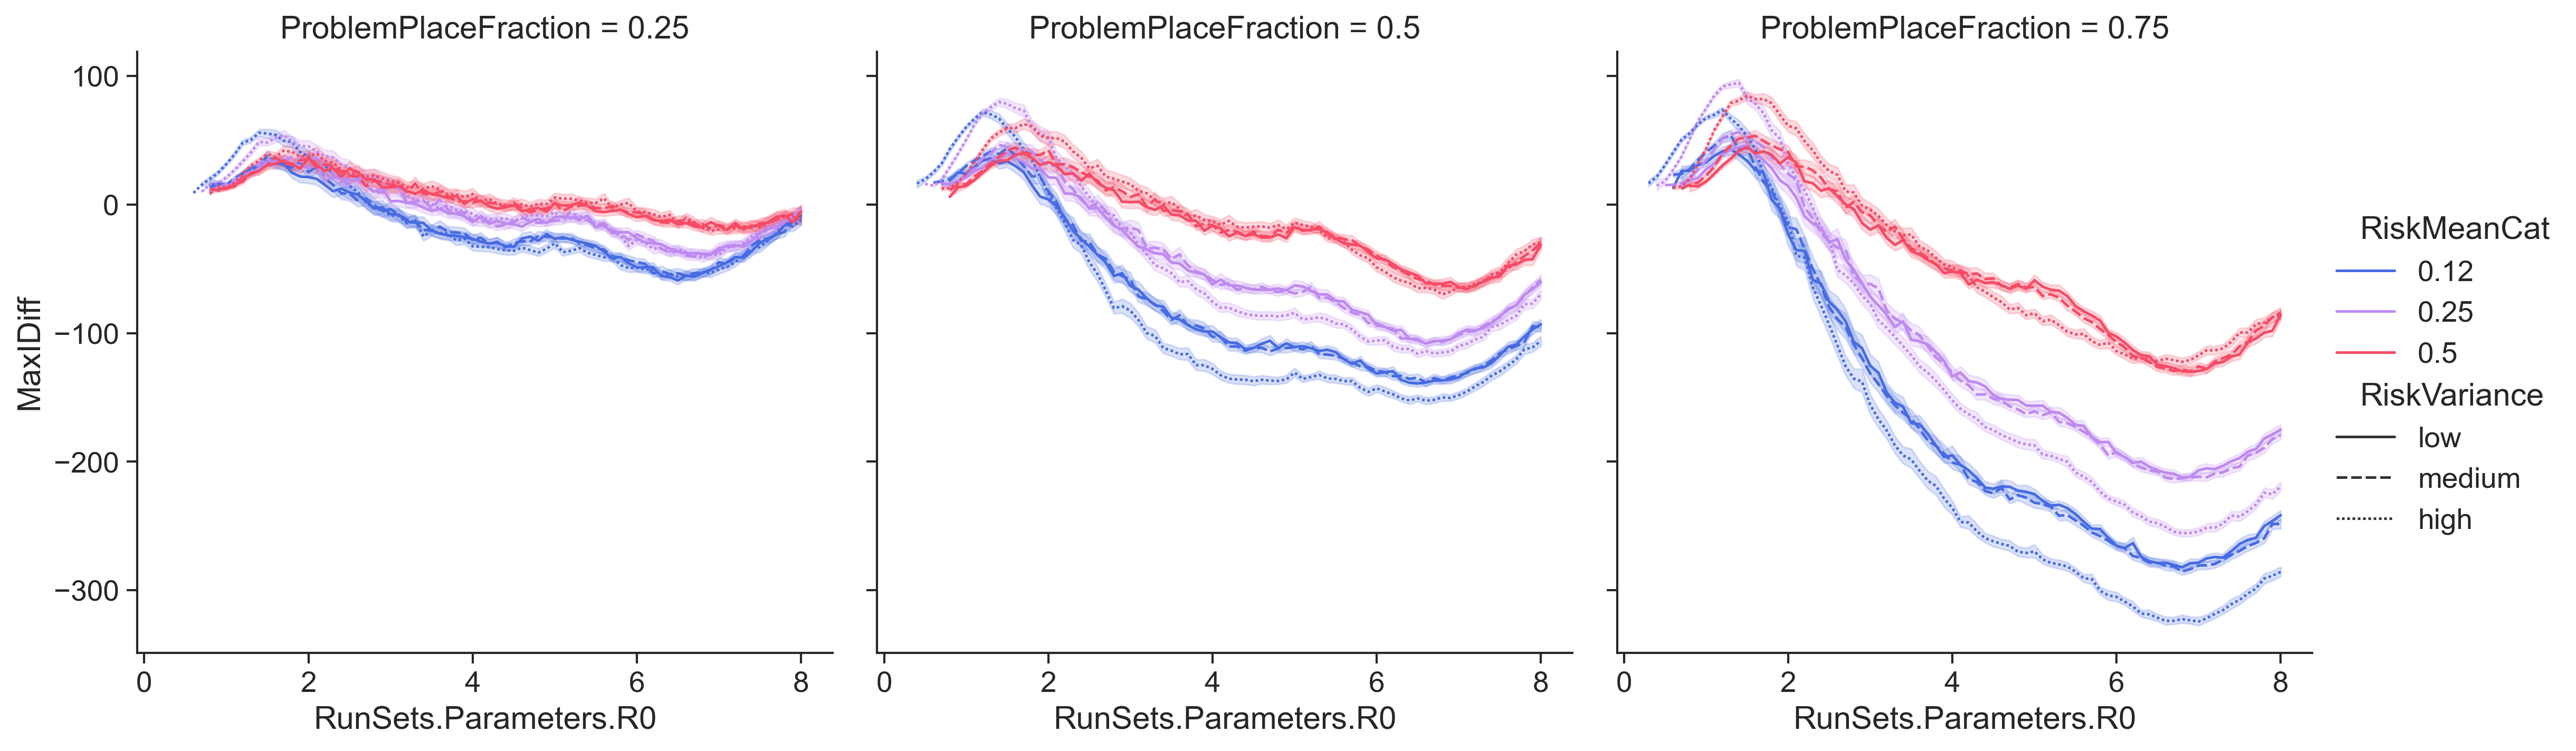
\includegraphics{images/MaxISim.png} 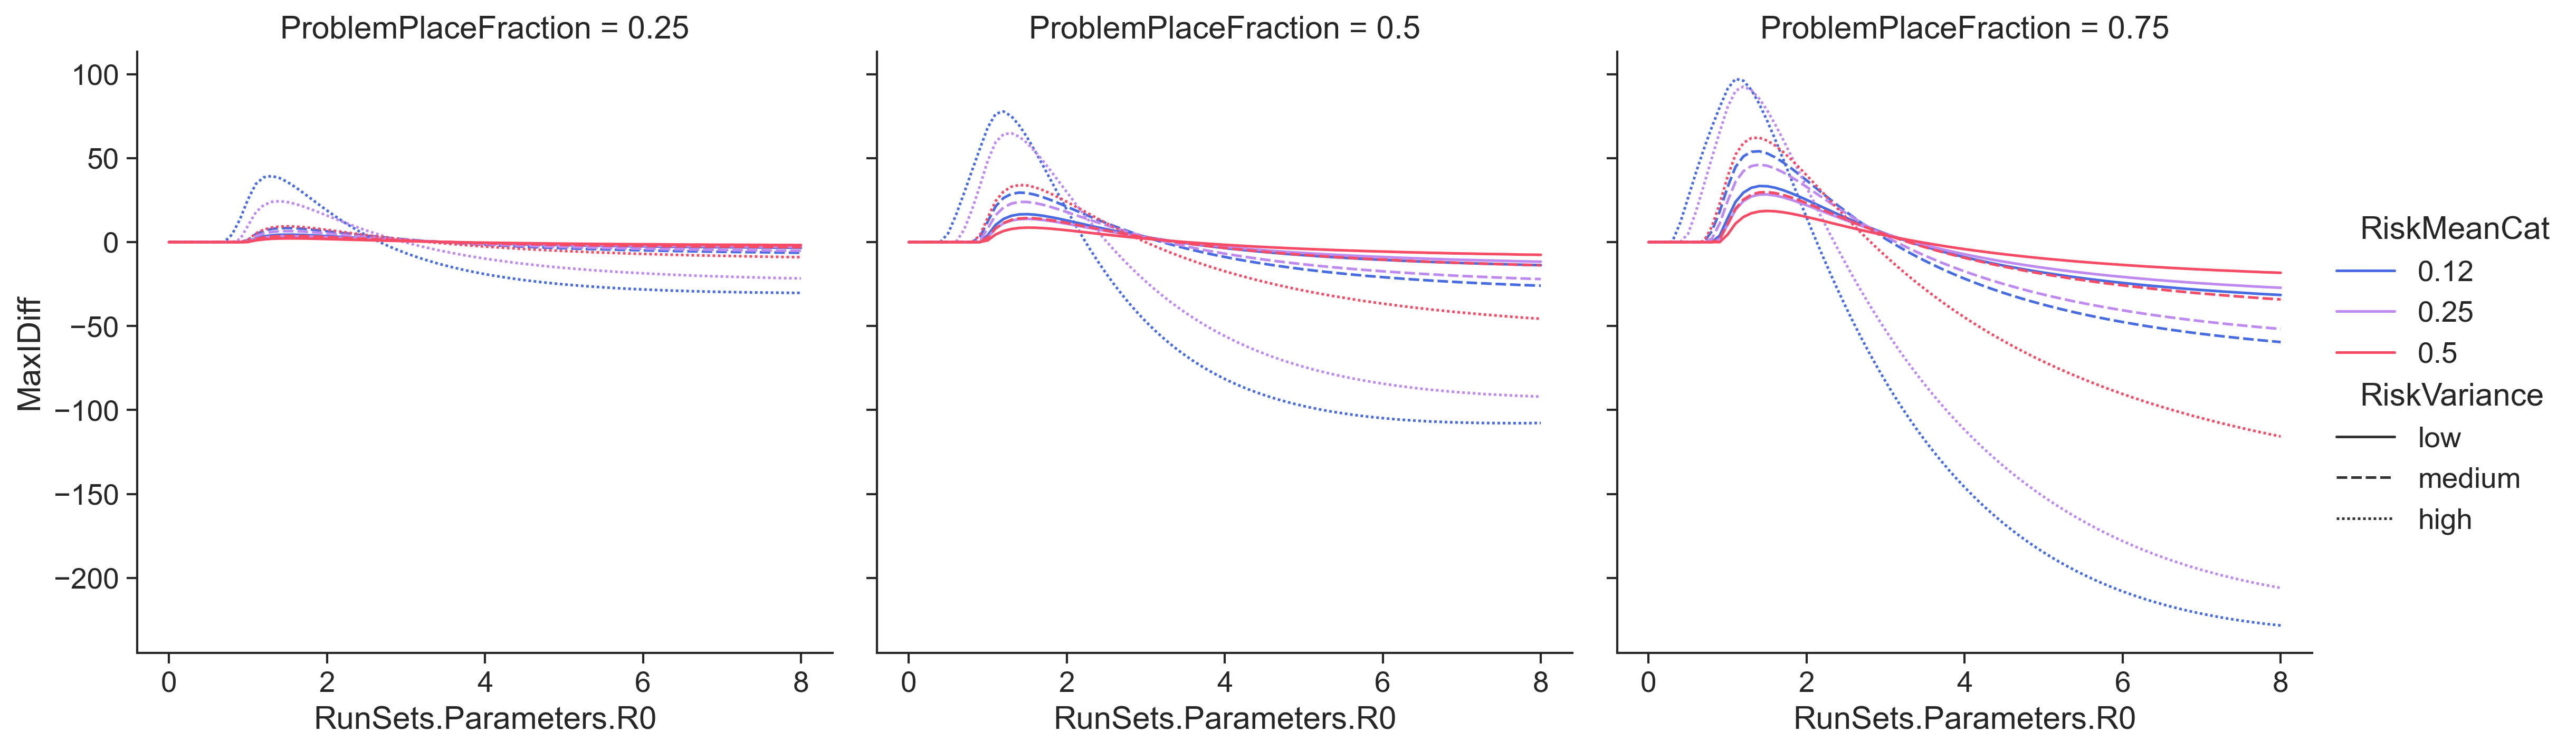
\includegraphics{images/MaxI.png}
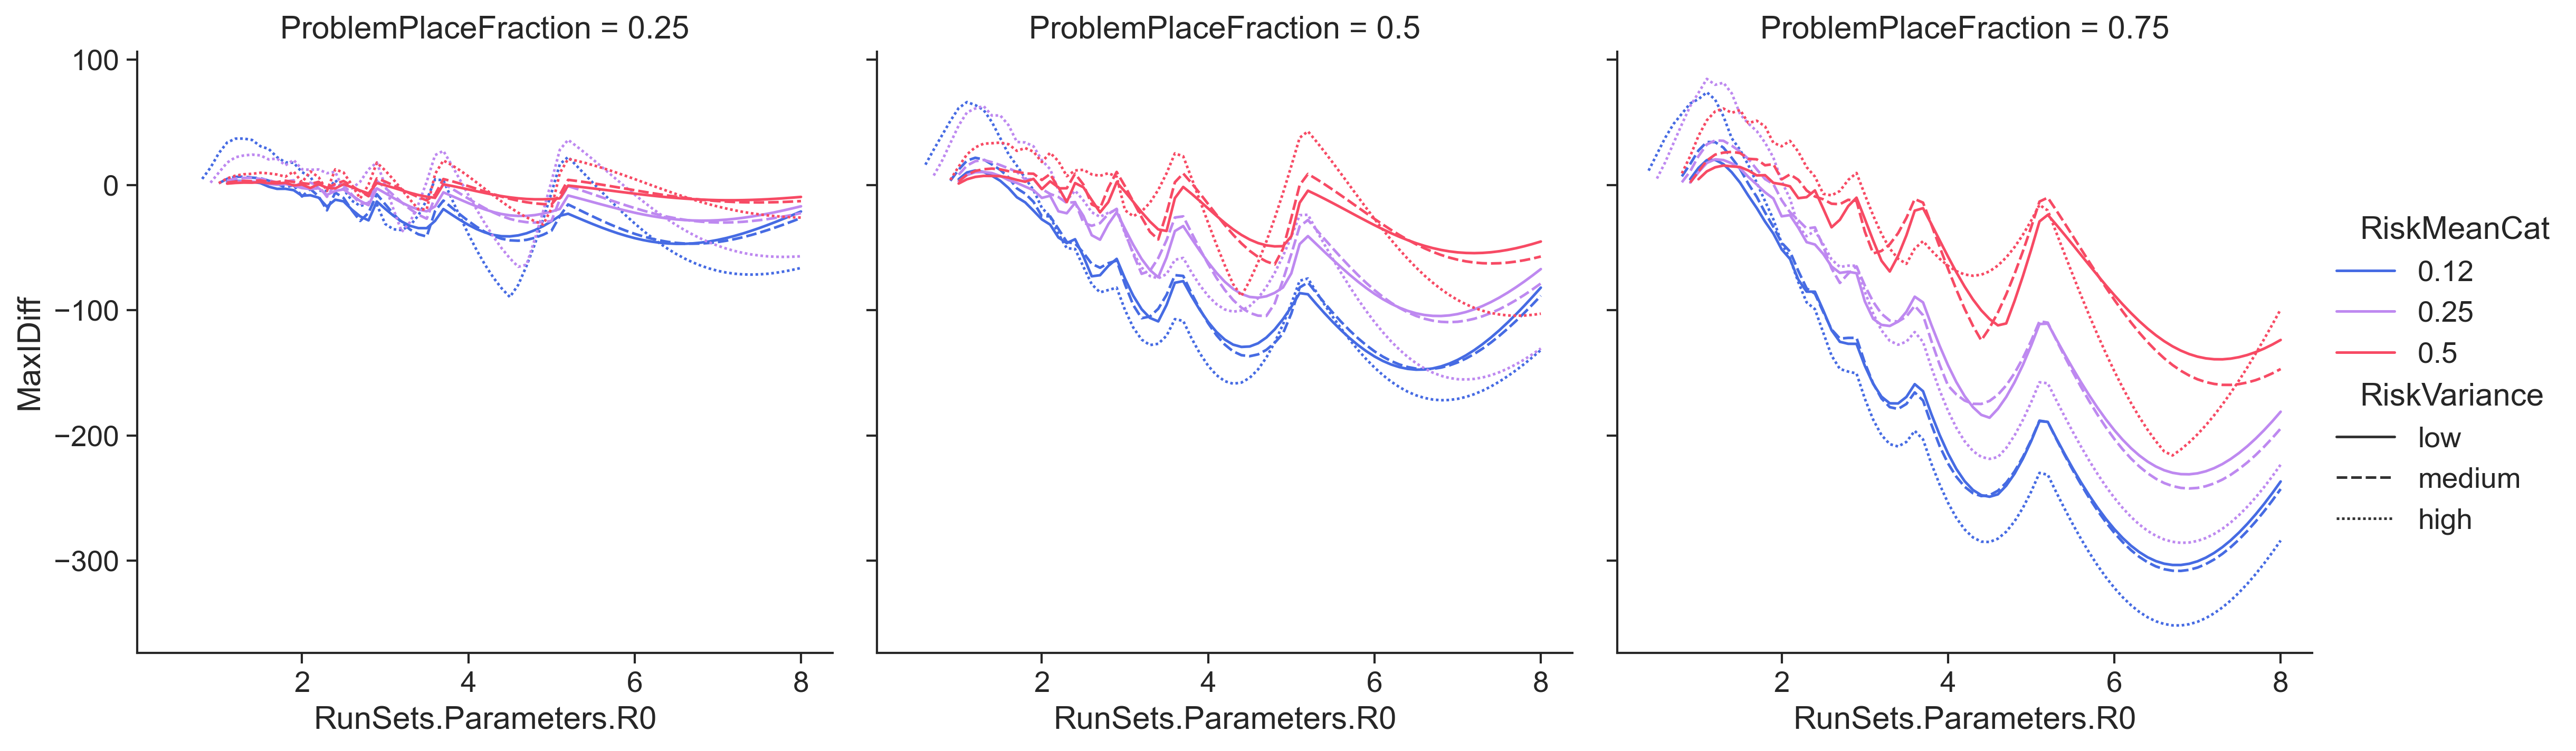
\includegraphics{images/MaxIDifference.png}

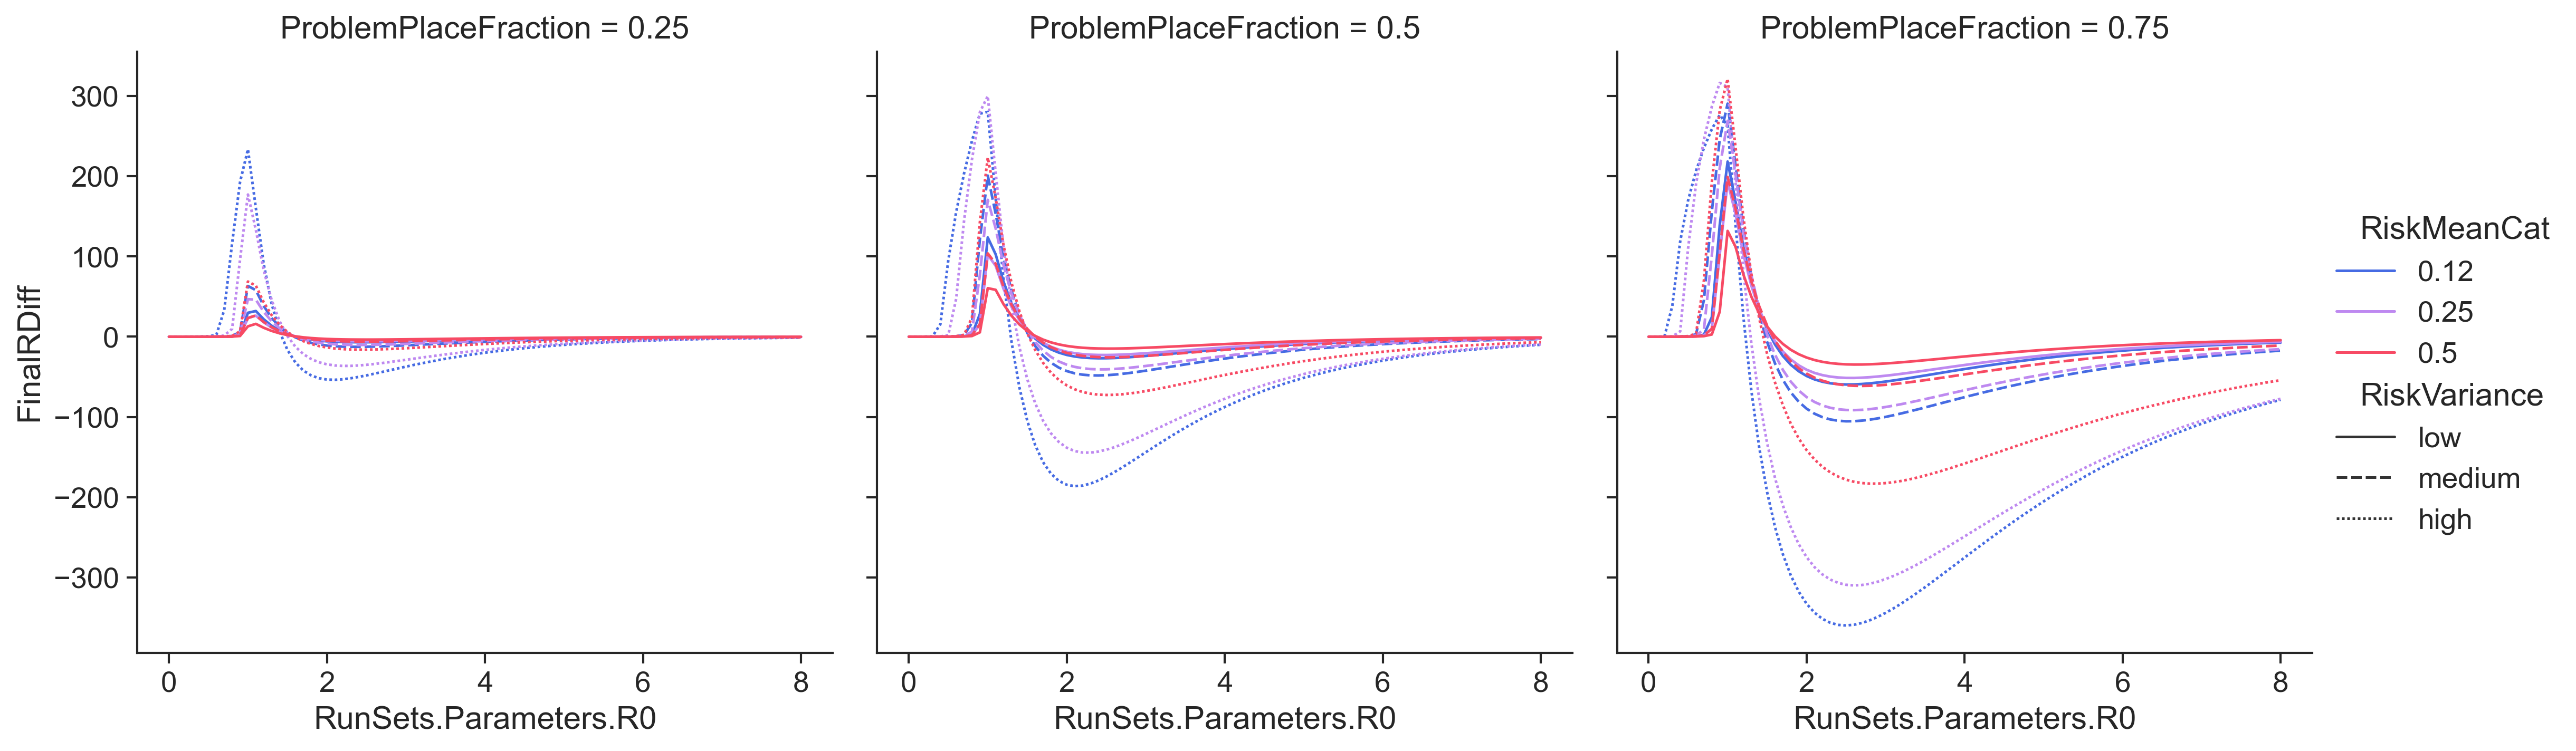
\includegraphics{images/FinalR.png}
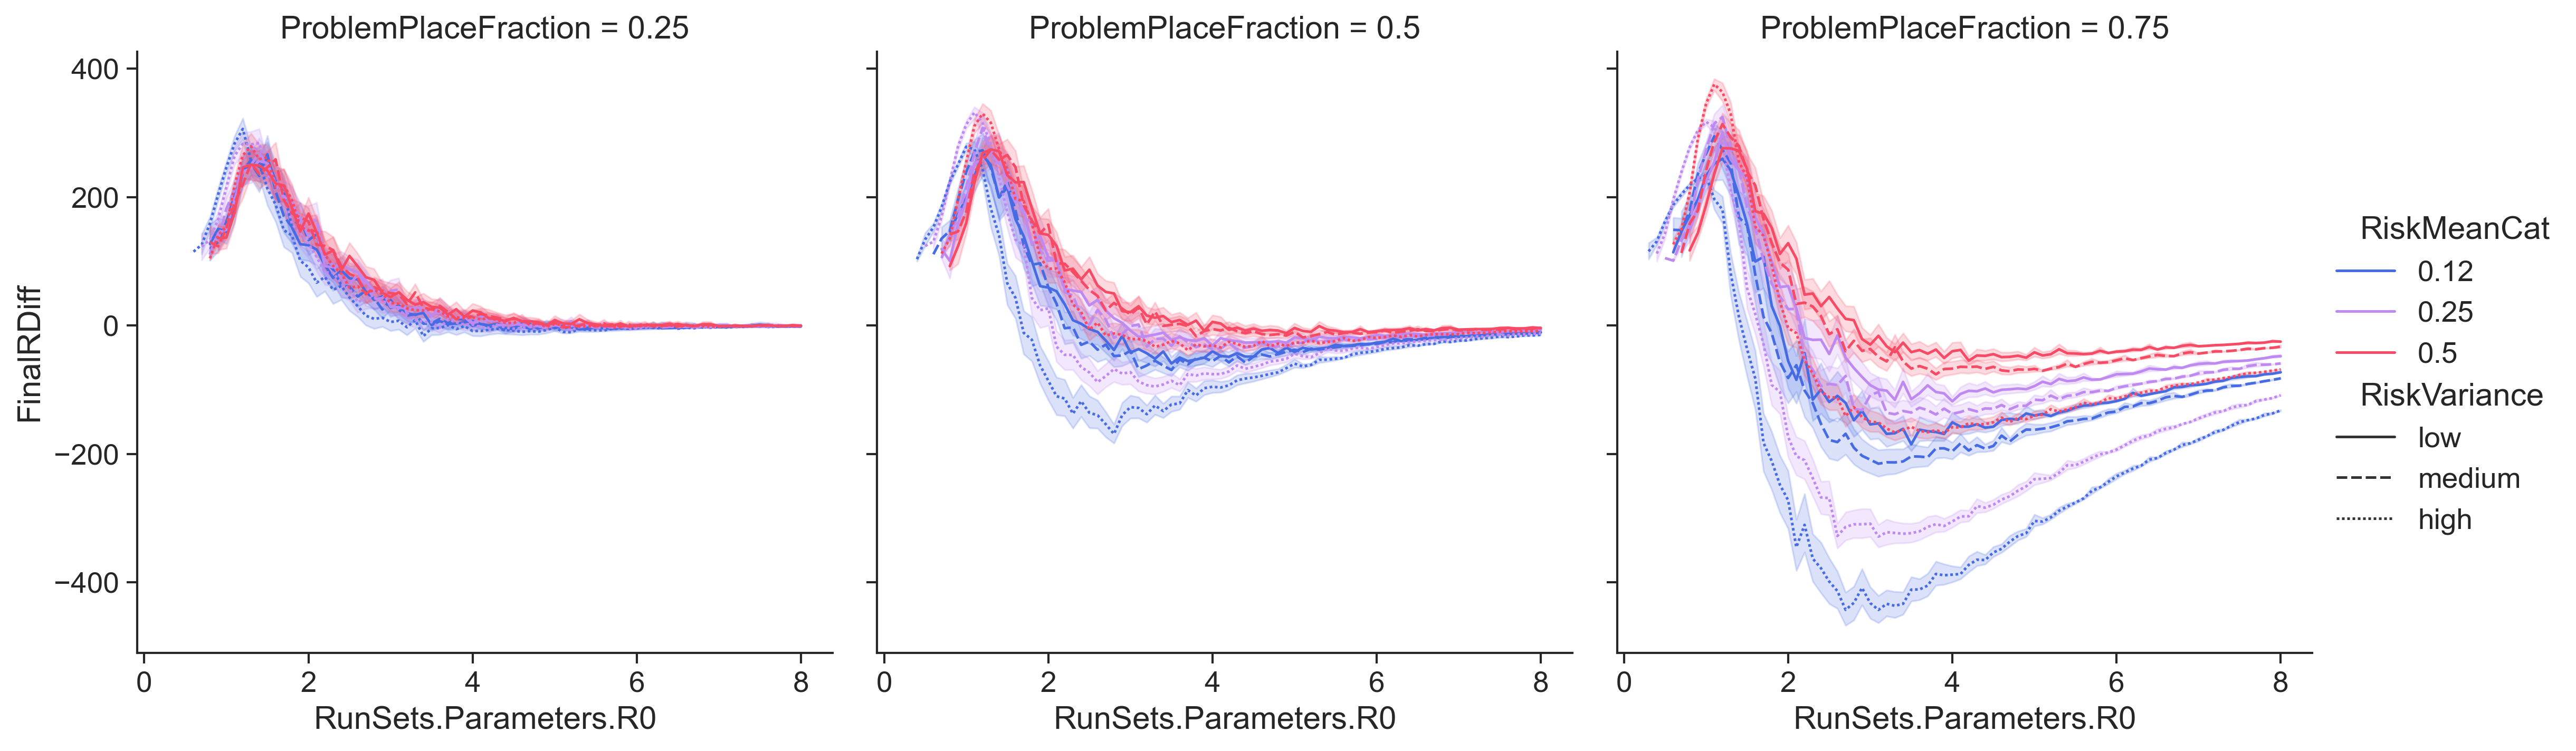
\includegraphics{images/FinalRSim.png}
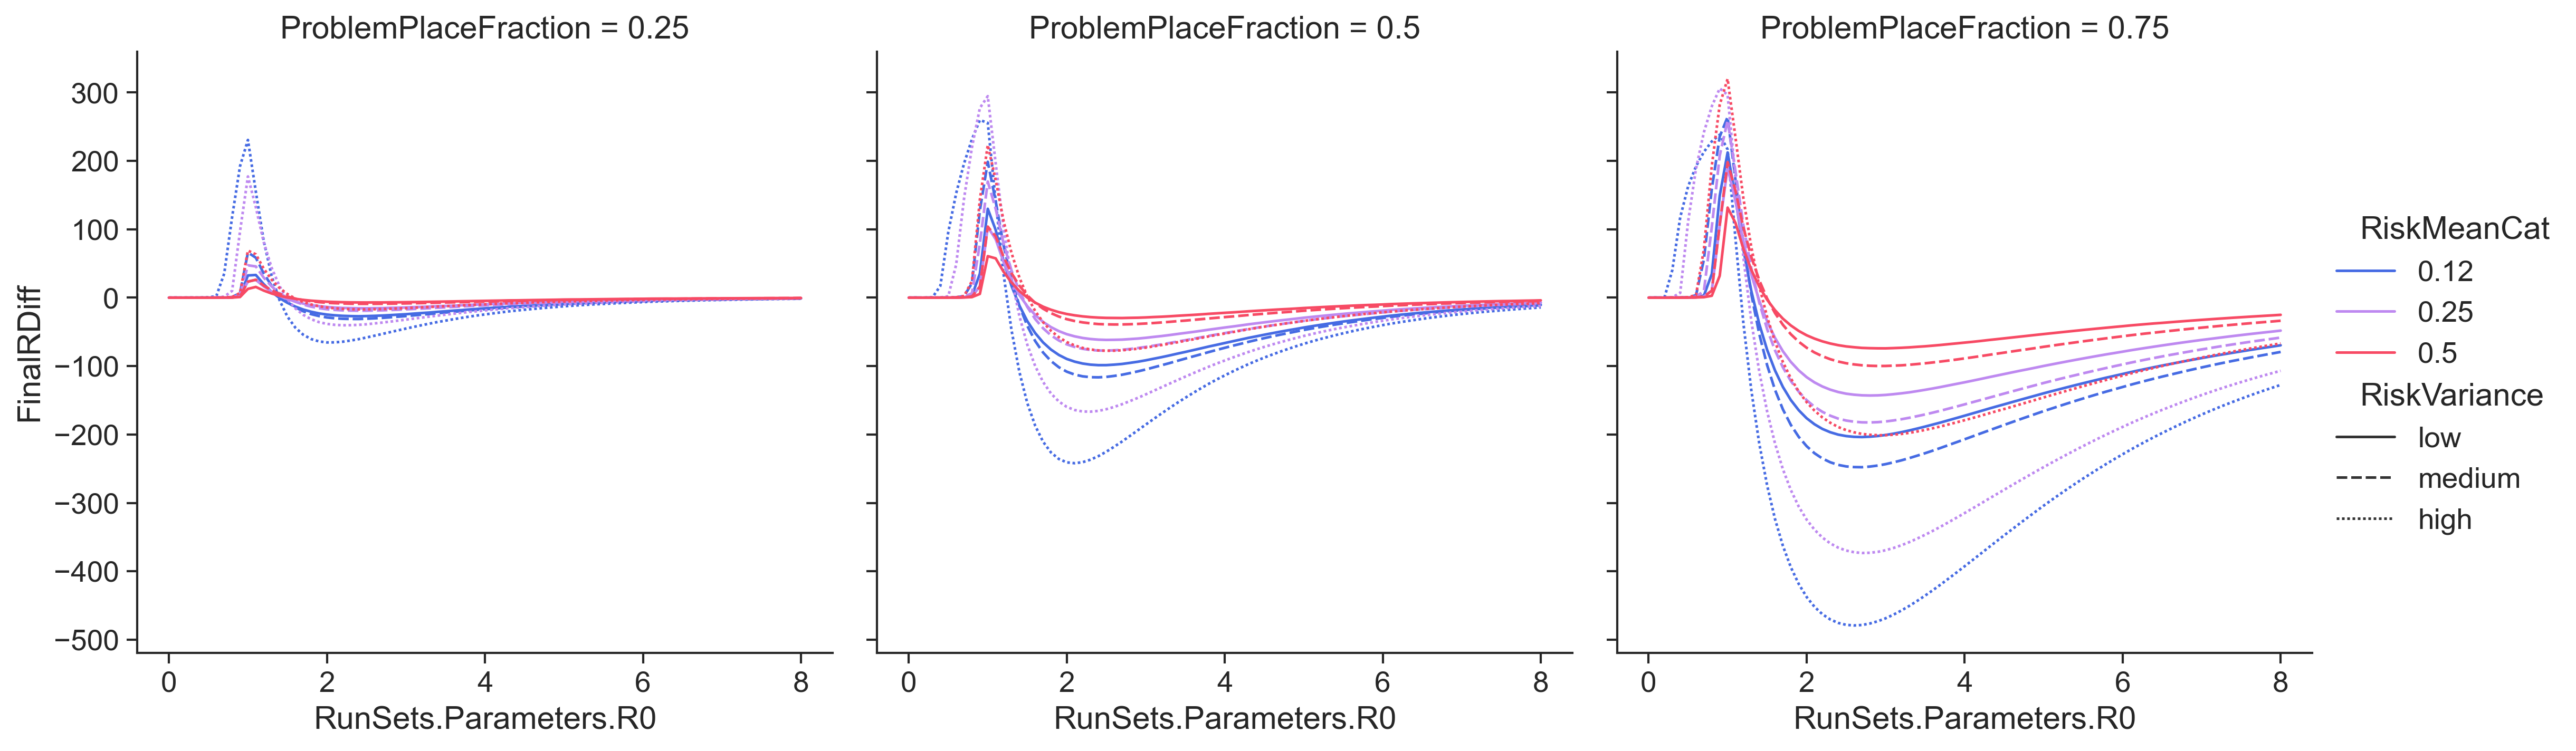
\includegraphics{images/FinalRDifference.png}
